\documentclass{article}


% if you need to pass options to natbib, use, e.g.:
%     \PassOptionsToPackage{numbers, compress}{natbib}
% before loading neurips_2024


% ready for submission
\usepackage{icml2024/icml2024}


% to compile a preprint version, e.g., for submission to arXiv, add add the
% [preprint] option:
%     \usepackage[preprint]{neurips_2024}


% to compile a camera-ready version, add the [final] option, e.g.:
%     \usepackage[final]{neurips_2024}


% to avoid loading the natbib package, add option nonatbib:
%    \usepackage[nonatbib]{neurips_2024}


\usepackage[utf8]{inputenc} % allow utf-8 input
\usepackage[T1]{fontenc}    % use 8-bit T1 fonts
\usepackage{url}            % simple URL typesetting
\usepackage{booktabs}       % professional-quality tables
\usepackage{amsfonts}       % blackboard math symbols
\usepackage{nicefrac}       % compact symbols for 1/2, etc.
\usepackage{microtype}      % microtypography
\usepackage{xcolor}         % colors

%\usepackage{amsmath, amsthm, amssymb}

\usepackage{expl3}  %
\ExplSyntaxOn
  \let\cstostr\cs_to_str:N
\ExplSyntaxOff
\usepackage{ifthen}
\usepackage{pgffor}

\usepackage[acronym,nowarn,section,nonumberlist]{glossaries}
\glsdisablehyper  %
\makeglossaries

\setacronymstyle{long-short}

\loadglsentries{preamble/acronyms.tex}

\usepackage{bm}
\usepackage[T1]{fontenc}  %
\usepackage[type1]{libertine}
\usepackage{mathtools}
\usepackage{tcolorbox}
\usepackage[makeroom]{cancel}   %
\usepackage{algorithm}
\usepackage{algpseudocode}


\usepackage{enumitem}

\usepackage{multirow}
\usepackage{array}
\usepackage{makecell}

%!TEX root = ckn-inv-nips.tex

\newcommand\st{~~~\text{s.t.}~~~}
\def\f{\tilde{f}}
\def\eg{\emph{e.g.}}
\def\ie{\emph{i.e.}}
\def\Hcal{{\mathcal H}}
\def\Kcal{{\mathcal K}}
\def\Fcal{{\mathcal F}}
\def\Pcal{{\mathcal P}}
\def\Xcal{{\mathcal X}}
\def\Real{{\mathbb R}}
%\def\vs{\vspace*{-0.1cm}}
\def\vs{}
%\def\kmone{k-1}
\def\kmone{k\text{--}1}
\def\kmtwo{k\text{--}2}
\def\nmone{n\text{--}1}
\def\defin{:=}

\def\x{{\mathbf x}}
\def\L{{\cal L}}
\def\R{{\mathbb R}}
\def\N{{\mathbb N}}
\def\Z{{\mathbb Z}}
\def\Hc{{\mathcal H}}
\def\Hcbar{\bar{\mathcal H}}
\def\activ{\sigma}

\DeclareMathOperator{\Tr}{Tr}
\DeclareMathOperator{\conv}{\textbf{conv}}
\DeclareMathOperator{\dom}{\textbf{dom}}
\DeclareMathOperator{\diag}{diag}
\DeclareMathOperator{\prox}{prox}
\DeclareMathOperator{\vect}{span}
\DeclareMathOperator{\Var}{Var}
\DeclareMathOperator{\cov}{cov}
\DeclareMathOperator{\E}{\mathbb{E}}
\DeclareMathOperator{\1}{\mathbbm{1}}

\newtheorem{theorem}{Theorem}
\newtheorem{proposition}[theorem]{Proposition}
% \newtheorem{lemma}[theorem]{Lemma}
% \newtheorem{corollary}[theorem]{Corollary}

\newtheorem{appxproposition}{Proposition}[section]
\newtheorem{appxtheorem}{Theorem}[section]
\newtheorem{appxlemma}{Lemma}[section]
\newtheorem{appxcorollary}{Corollary}[section]


\usepackage[hidelinks]{hyperref}       % hyperlinks

\title{The GAN is dead; long live the GAN!\\A Modern Baseline GAN}


% The \author macro works with any number of authors. There are two commands
% used to separate the names and addresses of multiple authors: \And and \AND.
%
% Using \And between authors leaves it to LaTeX to determine where to break the
% lines. Using \AND forces a line break at that point. So, if LaTeX puts 3 of 4
% authors names on the first line, and the last on the second line, try using
% \AND instead of \And before the third author name.


\begin{icmlauthorlist}
\icmlauthor{Yair Schiff}{cornell}
\icmlauthor{Chia-Hsiang Kao}{cornell}
\icmlauthor{Aaron Gokaslan}{cornell}
\icmlauthor{Tri Dao}{princeton}
\icmlauthor{Albert Gu}{cmu}
\icmlauthor{Volodymyr Kuleshov}{cornell}
\end{icmlauthorlist}

\icmlaffiliation{cornell}{Department of Computer Science, Cornell University, New York, NY USA}

\icmlkeywords{Machine Learning, Deep Learning, Language Modeling, Foundation Models, Genomics}

\vskip 0.3in
]
\begin{document}


\maketitle



\begin{abstract}
Language models (LMs), like other neural networks, often favor shortcut heuristics based on surface-level patterns.
Although LMs behave like n-gram models early in training, they must eventually learn hierarchical syntactic representations to correctly apply grammatical rules out-of-distribution (OOD).
In this work, we use case studies of English grammar to explore how complex, diverse training data drives models to generalize OOD. We construct a framework that unifies our understanding of random variation with training dynamics, rule selection with memorization, and data diversity with complexity. 
We show that these factors are nuanced, and that intermediate levels of diversity and complexity lead to inconsistent behavior across random seeds and to unstable training dynamics. 
Our findings emphasize the critical role of training data in shaping generalization patterns and illuminate how competing model strategies lead to inconsistent generalization outcomes across random seeds. Code is available at \url{https://github.com/sunnytqin/concept_comp.git}.

\end{abstract}

\section{Introduction}
\label{sec:introduction}

\begin{wrapfigure}{r}{0.5\textwidth}
\vspace{-6mm}
\begin{center}
    \includegraphics[width=0.5\textwidth]{images/cover.pdf}
  \end{center}
  \vspace{-4mm}
  \caption{\textbf{Overview of \implname.} In training, we tune the singular values of the weight matrices to generate a set of ``expert'' vectors specializing in different tasks. In inference, a two-pass process is adopted where the first applies the expert and the second generates the answer.}
  \label{fig:cover}
  \vspace{-4mm}
\end{wrapfigure}

Self-adaptive large language models (LLMs) would represent a significant advancement in artificial intelligence, enabling real-time adaptation to various tasks and contexts.
While compositionality and scalability are crucial for effective adaptation, current LLM training methodologies fall short of achieving both these properties simultaneously.
Our research aims to present a solution to address these gaps.

In principle, the first step toward achieving self-adaptive LLMs can be realized through the development of specialized expert modules, each fine-tuned~\citep{kaplan2020scaling} via techniques such as low-rank adaptation (LoRA)~\citep{hu2021lora}. 
However, several challenges need to be addressed to make this approach both scalable and compositional: (1) multiple expert modules significantly increase the number of parameters; (2) expert modules are often prone to overfitting; and (3) flexible composition of these experts is still an open problem.

To overcome these limitations, we first propose \svdacro, a novel parameter-efficient fine-tuning (PEFT) method to obtain effective building blocks for self-adaptation.
\svdacro works by extracting and selectively tuning only the singular values within the model's weight matrices.
By focusing on this essential and principled parameterization, our approach mitigates the risk of overfitting, drastically reduces computational demands, and allows for inherent compositionality.

We then introduce our full \implname framework, which entails a two-pass inference mechanism to produce dynamically adapted weights targeted for the test-time conditions (Figure~\ref{fig:cover}).
We design three different adaptation strategies that can be used within \implname, which we show provide monotonic performance benefits with increasing access to the test-time conditions.
We evaluate \svdacro and the full \implname framework through extensive experiments across a diverse range of LLMs and tasks.
\svdacro outperforms traditional efficient fine-tuning methods like LoRA on domain-specific datasets with far fewer parameters. 
\implname further improves performance, even for out-of-distribution tasks like visual QA. 
Our analysis even shows that \implname allows the reuse of \svdacro experts across different LLMs. In summary, our key technical contributions are: 
\vspace{-2mm}
\begin{itemize}
\item The development of \implname as a pivotal self-adaptation framework for LLMs, providing a blueprint to adapt the behavior of LLMs from a growing set of pre-trained skills.
\item The introduction of \svdacro, a novel PEFT method trainable with RL on small datasets, producing compact expert vectors with inherent compositionality.
\item The implementation of three adaptation strategies, effectively dispatching \svdacro-trained experts with properties designed to cope with different deployment scenarios.
\end{itemize}

\vspace{-2mm}


%------------------------------------------------------------------------
\section{Serving Two Masters: Stability and Diversity with RpGAN \texorpdfstring{$+ R_1+R_2$}{R-1R-2}}
%---An Improved Training Objective \vk{title can be tweaked; i recommend naming your new loss}}
% James Tompkin: I wrote 'serving two masters'. Note that 'serving two masters' is inherently a religious label; in the bible, Matthew writes that one cannot serve two masters (only God). In the traditions of monarchy (to which our title alludes in the procession of kings), a king had divine right and so avoided this problem of serving two masters (to serve God and to serve one's king is to serve two masters, except once we establish that kings are divine then this problem goes away as the same master - God - is then being served). I am not religious.
\label{sec:loss}

In defining a GAN objective, we tackle two challenges: stability and diversity. Some previous work deals with stability~\cite{sg1,sg2,sg3} and other previous work deals with mode collapse \cite{rgan}. To make progress in both, we combine a stable method with a simple regularizer that is grounded by theory.


\subsection{Traditional GAN}
A traditional GAN~\cite{gan,nowozin2016f} is formulated as a minimax game between a discriminator (or critic) $D_\psi$ and a generator $G_\theta$. Given real data $x\sim p_\mathcal{D}$ and fake data $x\sim p_\theta$ produced by $G_\theta$, the most general form of a GAN is given by:
\begin{align}
\begin{split}
\label{eq:gan}
\mathcal{L}(\theta,\psi)=\mathbb{E}_{z\sim p_z}\left[f\left(  D_\psi(G_\theta(z))\right)\right]+\mathbb{E}_{x\sim p_\mathcal{D}}\left[f\left( -D_\psi(x) \right)\right]
\end{split}
\end{align}
\noindent where $G$ tries to minimize $\mathcal{L}$ while $D$ tries to maximize it. The choice of $f$ is flexible~\cite{lsgan,hingegan}. In particular, $f(t) = -\log(1+e^{-t})$ recovers the classic GAN by Goodfellow~\etal~\cite{gan}. For the rest of this work, this will be our choice of $f$~\cite{nowozin2016f}.

% It is shown that Eq.\ref{eq:gan} is actually convex if we can directly optimize $p_\theta$~\cite{gan,rpgan}. Though in practice, the empirical GAN loss moves fake samples past the decision boundary induced by $D$ rather than updating the density function $p_\theta$ directly. This turns out to be a much harder problem that is susceptible to two common failure cases: mode collapse/dropping\footnote{Mode collapse and mode dropping are technically two related yet distinct problems. We use these two terms interchangeably hereafter to refer to the general problem where $\supp p_\theta$ fails to fully cover $\supp p_\mathcal{D}$.} and non-convergence. \vk{Minor thing: could provide a bit more information (1 sentence) on mode dropping and collapse}
It has been shown that Equation~\ref{eq:gan} has convex properties when $p_\theta$ can be optimized directly~\cite{gan,rpgan}. However, in practical implementations, the empirical GAN loss typically shifts fake samples beyond the decision boundary set by $D$, as opposed to directly updating the density function $p_\theta$. This deviation leads to a significantly more challenging problem, characterized by susceptibility to two prevalent failure scenarios: mode collapse/dropping\footnote{While mode collapse and mode dropping are technically distinct issues, they are used interchangeably in this context to describe the common problem where $\supp(p_\theta)$ does not comprehensively cover $\supp(p_\mathcal{D})$. Mode collapse refers to the generator producing a limited diversity of samples (i.e., one image for the entire distribution), whereas mode dropping involves the generator failing to represent certain modes of the data distribution (ignoring entire subsets of the training distribution).} and non-convergence.



\subsection{Relativistic \texorpdfstring{$f$-GAN}{f-GAN}}
% We adopt relativistic pairing GAN (RpGAN) by Jolicoeur-Martineau~\etal~\cite{rgan} as the main GAN loss. 
% Sun~\etal showed that RpGAN is especially effective against mode dropping~\cite{rpgan} as the loss landscape of RpGAN contains no local minima that correspond to mode dropping solutions. 
% Next, we apply zero-centered gradient penalties~\cite{r1,r1r2} to RpGAN. Gradient penalty is a well known technique that stabilizes GAN training~\cite{wgan-gp,r1r2,r1} and has been proven to be crucial to GAN convergence~\cite{r1}. As our contribution to the theory, we follow Mescheder~\etal~\cite{r1} and prove that gradient-penalized RpGAN enjoys the same guarantee of local convergence as regularized classic GANs. In addition to theoretical guarantees, our empirical results suggest that gradient penalized RpGAN is sufficiently well-behaved, to the extent that allows us to remove all GAN tricks without encountering non-convergence or mode dropping.

We employ a slightly different minimax game named relativistic pairing GAN (RpGAN) by Jolicoeur-Martineau~\etal~\cite{rgan} to address mode dropping. The general RpGAN is defined as:
\begin{equation}
\label{eq:rpgan}
\mathcal{L}(\theta,\psi)=\mathbb{E}_{\substack{z\sim p_z\\x\sim p_\mathcal{D}}}\left[f\left(  D_\psi(G_\theta(z))-D_\psi(x) \right)\right]
\end{equation}
Although Eq.~\ref{eq:rpgan} differs only slightly from Eq.~\ref{eq:gan}, evaluating this critic difference has a fundamental impact on the landscape of $\mathcal{L}$. Since Eq.~\ref{eq:gan} merely requires $D$ to separate real and fake data, in the scenario where all real and fake data can be separated by a single decision boundary, the empirical GAN loss encourages $G$ to simply move all fake samples barely past this single boundary---this degenerate solution is what we observe as mode collapse/dropping. Sun~\etal~\cite{rpgan} characterize such degenerate solutions as bad local minima in the landscape of $\mathcal{L}$, and show that Eq.~\ref{eq:gan} has \emph{exponentially many} bad local minima. The culprit is the existence of a single decision boundary that naturally arises when real and fake data are considered in isolation. RpGAN introduces a simple solution by coupling real and fake data,~\ie a fake sample is critiqued by its realness \emph{relative to} a real sample, which effectively maintains a decision boundary in the neighborhood of \emph{each} real sample and hence forbids mode dropping. Sun~\etal~\cite{rpgan} show that the landscape of Eq.~\ref{eq:rpgan} contains no local minima that correspond to mode dropping solutions, and that every basin is a global minimum.


\subsection{Training Dynamics of RpGAN}
Although the RpGAN landscape result~\cite{rpgan} allows us to address mode dropping, the training dynamics of RpGAN have yet to be studied. The ultimate goal of Eq.~\ref{eq:rpgan} is to find the equilibrium $(\theta^*,\psi^*)$ such that $p_{\theta^*}=p_\mathcal{D}$ and $D_{\psi^*}$ is constant everywhere on $p_\mathcal{D}$. Sun~\etal~\cite{rpgan} show that $\theta^*$ is globally reachable along a non-increasing trajectory in the landscape of Eq.~\ref{eq:rpgan} under reasonable assumptions. However, the existence of such a trajectory does not necessarily mean that gradient descent will find it. Jolicoeur-Martineau~\etal show empirically that unregularized RpGAN does not perform well~\cite{rgan}. 

\vspace{1ex}
\noindent \textbf{Proposition~\upperRomannumeral{1}.} (Informal) \emph{Unregularized RpGAN does not always converge using gradient descent.}
%\vk{Propositions should ideally be made precise or in the worst case, say it's an informal statement (but then you still have to make it intuitively understandable)}
\vspace{1ex}

\noindent We confirm this proposition with a proof in Appendix B. 
% In summary, we follow Mescheder~\etal~\cite{r1} and inherit their DiracGAN counterexample to apply it to RpGAN. 
We show analytically that RpGAN does not converge for certain types of $p_\mathcal{D}$, such as ones that approach a delta distribution. Thus, further regularization is necessary to fill in the missing piece of a well-behaved loss.

\paragraph{Zero-centered gradient penalties.}
To tackle RpGAN non-convergence, we explore gradient penalties as the solution since it is proven that zero-centered gradient penalties (0-GP) facilitate convergent training for classic GANs~\cite{r1}. The two most commonly-used 0-GPs are $R_1$ and $R_2$:
\begin{equation}
\begin{aligned}
R_1(\psi)&=\frac{\gamma}{2}\mathbb{E}_{x\sim p_\mathcal{D}}\left[\left\| \nabla_x D_\psi \right \|^2\right]\\ 
R_2(\theta,\psi)&=\frac{\gamma}{2}\mathbb{E}_{x\sim p_\theta}\hspace{0.06cm}\left[\left\| \nabla_x D_\psi \right \|^2\right]
\end{aligned}
\end{equation}
$R_1$ penalizes the gradient norm of $D$ on real data, and $R_2$ penalizes the gradient norm of $D$ on fake data. Analysis on the training dynamics of GANs has thus far focused on local convergence~\cite{nagarajan2017gradient,gannum,r1},~\ie, whether the training at least converges when $(\theta,\psi)$ are in a neighborhood of $(\theta^*,\psi^*)$. In such a scenario, the convergence behavior can be analyzed~\cite{nagarajan2017gradient,gannum,r1} by examining the spectrum of the Jacobian of the gradient vector field $\left(-\nabla_\theta\mathcal{L},\nabla_\psi\mathcal{L} \right )$ at $(\theta^*,\psi^*)$. The key insight here is that when $G$ already produces the true distribution, we want $\nabla_x D=0$, so that $G$ is not pushed away from its optimal state, and thus the training does not oscillate. $R_1$ and $R_2$ impose such a constraint when $p_\theta=p_\mathcal{D}$. This also explains why earlier attempts at gradient penalties, such as the one-centered gradient penalty (1-GP) in WGAN-GP~\cite{wgan-gp}, fail to achieve convergent training~\cite{r1} as they still encourage $D$ to have a non-zero slope when $G$ has reached optimality.

Since the same insight also applies to RpGAN, 
we extend our previous analysis and show that:
% our goal is to extend the proof of Mescheder~\etal~\cite{r1} to RpGAN and show that:

\vspace{1ex}
\noindent \textbf{Proposition~\upperRomannumeral{2}.} (Informal) \emph{RpGAN with $R_1$ or $R_2$ regularization is locally convergent subject to similar assumptions as in} Mescheder~\etal~\cite{r1}.
\vspace{1ex}

In Appendix C, our proof similarly analyzes the eigenvalues of the Jacobian of the regularized RpGAN gradient vector field at $(\theta^*,\psi^*)$. We show that all eigenvalues have a negative real part; thus, regularized RpGAN is convergent in a neighborhood of $(\theta^*,\psi^*)$ for small enough learning rates~\cite{r1}.

%\vk{This paragraph is too verbose and feels like belongs to a prior work or discussion section} 
\paragraph{Discussion.}
Another line of work~\cite{r1r2} links $R_1$ and $R_2$ to instance noise~\cite{instancenoise} as its analytical approximation. Roth et al.~\cite{r1r2} showed that for the classic GAN~\cite{gan} by Goodfellow~\etal, $R_1$ approximates convolving $p_\mathcal{D}$ with the density function of $\mathcal{N}(0, \gamma I)$, up to additional weighting and a Laplacian error term. $R_2$ likewise approximates convolving $p_\theta$ with $\mathcal{N}(0, \gamma I)$ up to similar error terms. The Laplacian error terms from $R_1$, $R_2$ cancel when $D_\psi$ approaches $D_{\psi^*}$. We do not extend Roth~\etal's proof~\cite{r1r2} to RpGAN; however, this approach might provide complimentary insights to our work, which follows the strategy of Mescheder~\etal~\cite{r1}.

\subsection{A Practical Demonstration}

%\vk{i don't think that the rest of this section belongs in the methods section; i would first make it less verbose, then i would move large parts of it to the experiments, and i would summarize here in 1-2 sentences} 

We experiment with how well-behaved our loss is on StackedMNIST~\cite{pacgan} which consists of 1000 uniformly-distributed modes. The network is a small ResNet~\cite{resnet2} for $G$ and $D$ without any normalization layers~\cite{bn,gn,ln,in}.
Through the use of a pretrained MNIST classifier, we can explicitly measure how many modes of $p_\mathcal{D}$ are recovered by $p_\theta$. Furthermore, we can estimate the reverse KL divergence between the fake and real samples $D_\text{KL}\left(p_\theta\parallel p_\mathcal{D} \right)$ via the KL divergence between the categorical distribution of $p_\theta$ and the true uniform distribution.
\begin{figure}
\begin{floatrow}
\ffigbox{%
  \centering
  \includegraphics[width=0.48\textwidth]{figures/MNIST_loss.pdf}%
}{%
\caption{Generator $G$ loss for different objectives over training. Regardless of which objective is used, training diverges with only $R_1$ and succeeded with both $R_1$ and $R_2$. Convergence failure with only $R_1$ was noted by Lee et al.~\cite{vitgan}.}
\label{fig:mnist_loss_curve}
}
\capbtabbox{%
\centering
    \begin{tabular}{ l rrr }
        \toprule
        Loss & \# modes$\uparrow$ & $D_\text{KL}$$\downarrow$ \\
        \midrule
        RpGAN $+ R_1+R_2$ & $\mathbf{1000}$ & $\mathbf{0.0781}$ \\
        GAN $+ R_1+R_2$ & $693$ & $0.9270$ \\
        RpGAN $+ R_1$ & Fail & Fail \\
        GAN $+ R_1$ & Fail & Fail \\
        \bottomrule
    \end{tabular}
}{%
    \caption{StackedMNIST~\cite{pacgan} result for each loss function. The maximum possible mode coverage is 1000. ``Fail'' indicates that training diverged early on.}
    \label{tab:loss}
}
\end{floatrow}
\end{figure}

%For our initial experiments, we adopt a small ResNet~\cite{resnet2} architecture without any normalization layer~\cite{bn,gn,ln,in} for $G$ and $D$. 
A conventional GAN loss with $R_1$, as used by Mescheder et al.~\cite{r1} and the StyleGAN series~\cite{sg1, sg2, sg3}, diverges quickly (Fig.~\ref{fig:mnist_loss_curve}). Next, while theoretically sufficient for local convergence, RpGAN with only $R_1$ regularization is also unstable and diverges quickly\footnote{Varying $\gamma$ from 0.1 to 100 does not stabilize training.}. In each case, the gradient of $D$ on fake samples explodes when training diverges. With both $R_1$ and $R_2$, training becomes stable for both the classic GAN and RpGAN. Now stable, we can see that the classic GAN suffers from mode dropping, whereas RpGAN achieves full mode coverage (Tab.~\ref{tab:loss}) and reduces $D_\text{KL}$ from 0.9270 to 0.0781. As a point of contrast, StyleGAN~\cite{sg1,sg2,sg2ada,sg3} uses the minibatch standard deviation trick to reduce mode dropping, improving mode coverage from 857 to 881 on StackedMNIST\footnote{These numbers are from Karras~\etal~\cite{pggan}, Table 4. "857" corresponds to a low-capacity version of a progressive GAN and "881" adds the minibatch standard deviation trick. Further comparisons via loss curves are difficult since progressive GAN is a substantially different model than the small ResNet we use for this experiment.} and with barely any improvement on $D_\text{KL}$~\cite{pggan}.

%With training instability out of our way, we are ready to examine quantitatively how our new loss performs compared to existing work~\cite{r1,pggan,sg2}. While with $R_1$ and $R_2$ in conjunction training is successful for both the classic GAN~\cite{gan} and RpGAN~\cite{rgan}, we see in Table~\ref{tab:loss} that the classic GAN suffers from mode dropping. In contrast, RpGAN not only achieves full mode coverage, more notably, it drastically reduces $D_\text{KL}$ from 0.927 to 0.0781, indicating a considerably more faithful reconstruction of $p_\mathcal{D}$. 

% Instead of modifying the loss function, the StyleGAN family~\cite{sg1,sg2,sg2ada,sg3} relies on a trick called minibatch standard deviation~\cite{pggan} to combat mode dropping. It is shown in~\cite{pggan} that minibatch standard deviation can only slightly improve mode coverage from 857 to 881 on StackedMNIST and it shows barely any improvement on $D_\text{KL}$. 
% RpGAN in comparison improves mode coverage from 693 to 1000 and reduces $D_\text{KL}$ by one magnitude. 
%This shows that RpGAN is not only more principled against mode dropping in theory, but more effective in practice too. 
% We show in Section.\ref{sec:exp} that with architectural improvements in Section.\ref{sec:roadmap}, we can further improve $D_\text{KL}$ on StackedMNIST and even beat likelihood-based models. For the rest of this work, RpGAN $+ R_1+R_2$ will be our loss function.

% We start with RpGAN with only $R_1$ regularization since theoretically this is sufficient for local convergence. Contrary to our expectations, the training process utilizing this loss function exhibited significant instability and rapidly diverged. We experimented with various values of $\gamma$, ranging from 0.1 to 100; however, none succeeded in stabilizing the training. Furthermore, we explored integrating the conventional GAN loss combined with $R_1$, as commonly employed in the work of Mescheder et al.~\cite{r1} and the StyleGAN series~\cite{sg1, sg2, sg3}. Notably, this configuration led to even quicker divergence than the $R_1$ regularized RpGAN.
%To our surprise, training with this loss has been quite unstable and it diverges very quickly. We tried different $\gamma$ values ranging from 0.1 to 100 but none could prevent training from diverging. We also experiment with the combination of classic GAN and $R_1$, this is the widely adopted GAN loss in Mescheder~\etal~\cite{r1} and the StyleGAN family~\cite{sg1,sg2,sg3}, yet this loss diverges even faster than $R_1$ regularized RpGAN. 

% Upon closer inspection, we notice that the gradient of $D$ on fake samples explodes when training diverges. This motivates us to also apply $R_2$ regularization along with $R_1$, we see in Figure~\ref{fig:mnist_loss_curve} that with both $R_1$ and $R_2$, training becomes stable for both the classic GAN and RpGAN. 

$R_1$ alone is not sufficient for globally-convergent training. While a theoretical analysis of this is difficult, our small demonstration still provides insights into the assumptions of our convergence proof. 
In particular, the assumption that $(\theta,\psi)$ are sufficiently close to $(\theta^*,\psi^*)$ is highly unlikely early in training. In this scenario, if $D$ is sufficiently powerful, regularizing $D$ solely on real data is not likely to have much effect on $D$'s behavior on fake data and so training can fail due to an ill-behaved $D$ on fake data. This observation has been made by previous studies~\cite{r1gradexp, r1gradexpcvpr} specifically for empirical GAN training, that regularizing an empirical discriminator with only $R_1$ leads to gradient explosion on fake data due to the memorization of real samples.

% \vk{this is the key part that should be summarized in 1-2 sentences in this section: you find empirically and mathematically that both types of regularization are needed to make things work; then in the experiments section or in the appendix you provide results that show that it's the case}

Thus, the practical solution is to regularize $D$ on both real and fake data. The benefit of doing so can be viewed from the insight of Roth~\etal~\cite{r1r2}: that applying $R_1$ and $R_2$ in conjunction smooths both $p_\mathcal{D}$ and $p_\theta$ which makes learning easier than only smoothing $p_\mathcal{D}$. We also find empirically that with both $R_1$ and $R_2$ in place, $D$ tends to satisfy $\mathbb{E}_{x\sim p_\mathcal{D}}\left[\left\| \nabla_x D \right \|^2\right]\approx\mathbb{E}_{x\sim p_\theta}\left[\left\| \nabla_x D \right \|^2\right]$ even early in the training. Jolicoeur-Martineau~\etal~\cite{ganmmc} show that in this case $D$ becomes a maximum margin classifier---but if only one regularization term is applied, this does not hold. Additionally, having roughly the same gradient norm on real and fake data potentially reduces discriminator overfitting, as Fang~\etal~\cite{diggan} observe that the gradient norm on real and fake data diverges when $D$ starts to overfit.

% \vk{by the way, you will need a discussion of your regularization to other uses of this similar regularizer in the discussion or related work section}
% \begin{figure}
%     \centering
%     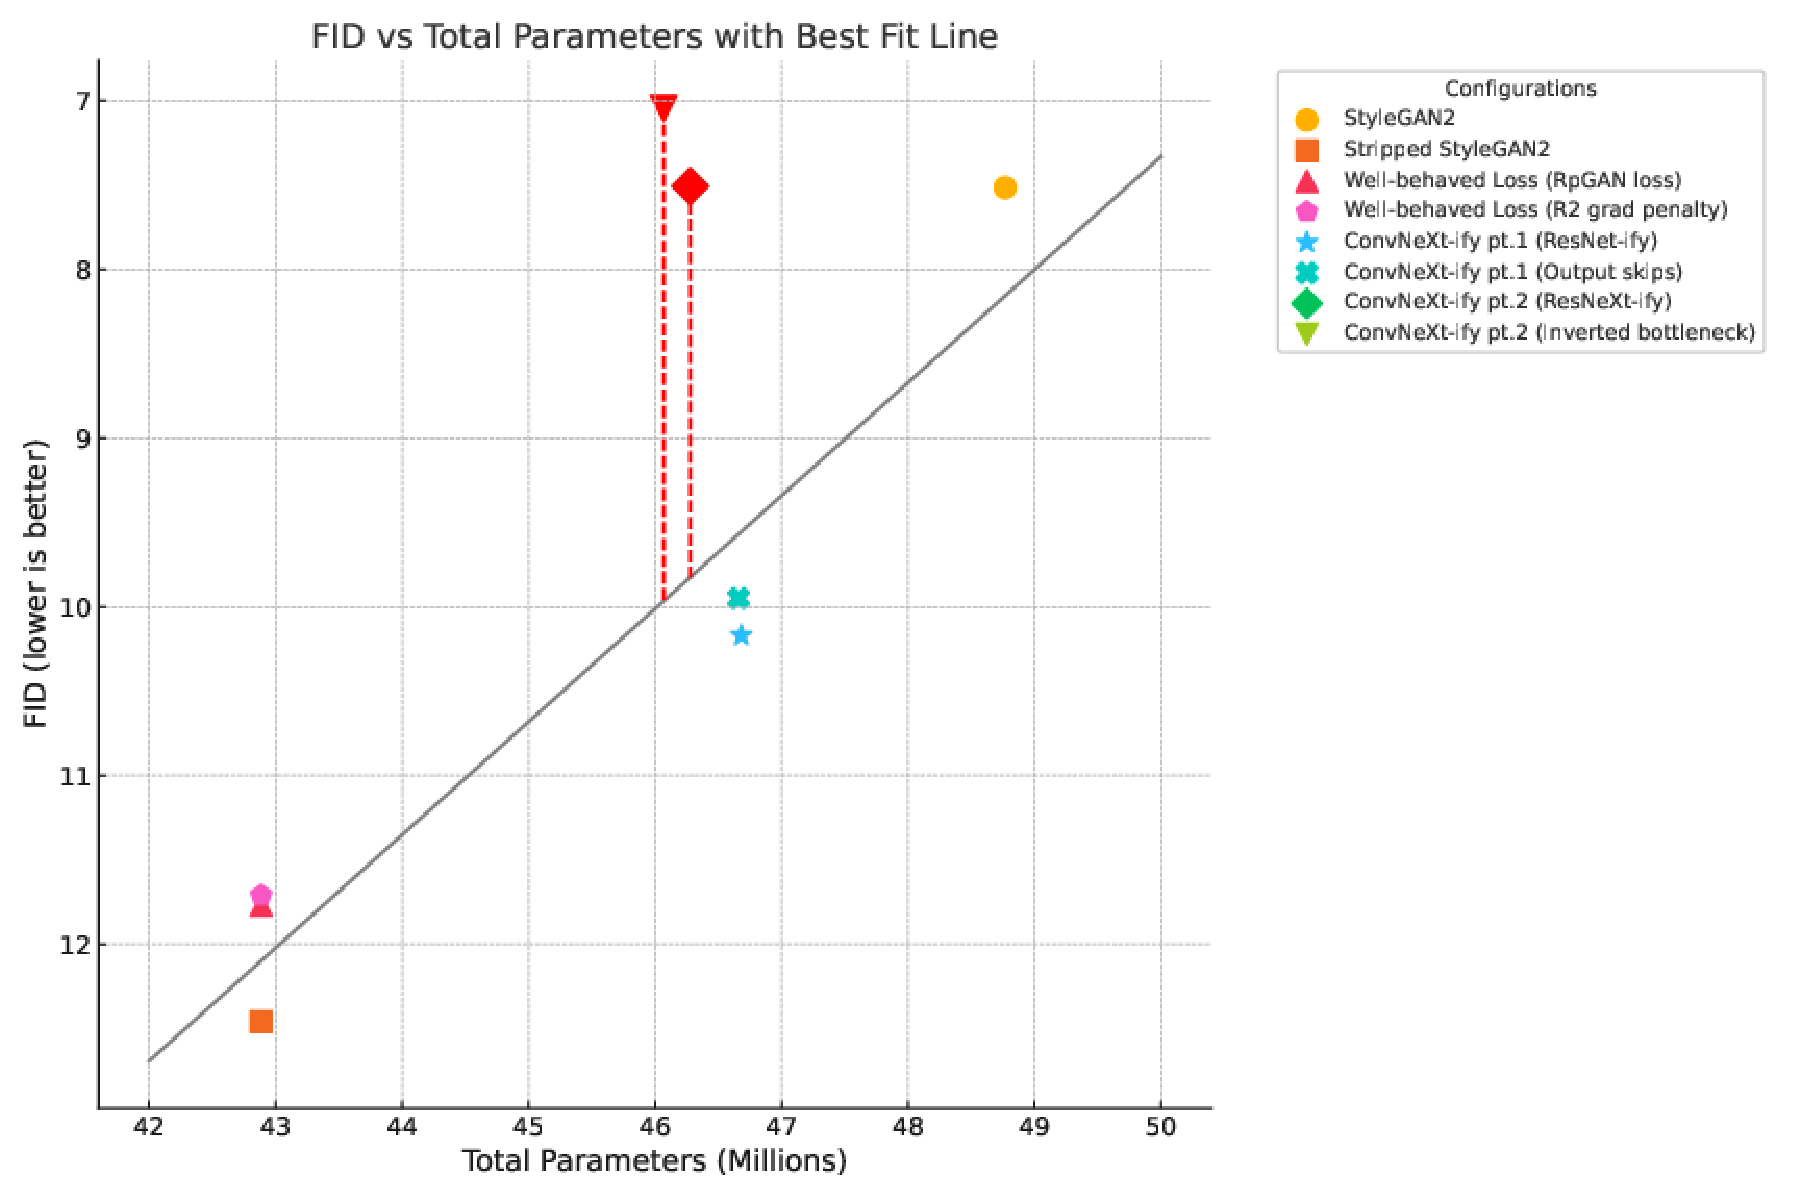
\includegraphics{figures/FID-vs-Params-Plot.eps}
%     \caption{This scatter-plot shows the FID performance of our model on FFHQ-256 vs the number of parameters when only trained for 5million steps}
%     \label{fig:fid-vs-params-ablation}
% \end{figure}


\section{A Roadmap to a New Baseline --- \modelName}
\label{sec:roadmap}

% \vk{What about naming the new GAN that is being proposed? SimpleGAN...?}\jt{R3GAN...?}

% \vk{My main comment about this section is that it reads like mix of methods and experiments: all the experimental details/results (e.g., we set the learning rate to $10^{-4}$) should be under experiments (but you can still describe the key important takeaways here, e.g., we need a smaller learning rate)}

The well-behaved RpGAN + $R_1$ + $R_2$ loss alleviates GAN optimization problems, and lets us proceed to build a minimalist baseline---\modelName---with recent network backbone advances in mind~\cite{convnext,metaformer}. Rather than simply state the new approach, we will draw out a roadmap from the StyleGAN2 baseline~\cite{sg2ada}. This model (Config A; identical to~\cite{sg2ada}) consists of a VGG-like~\cite{vgg} backbone for $G$, a ResNet $D$, a few techniques that facilitate style-based generation, and many tricks that serve as patches to the weak backbone. Then, we remove all non-essential features of StyleGAN2 (Config B), apply our loss function (Config C), and gradually modernize the network backbone (Config D-E).


We evaluate each configuration on FFHQ $256\times256$~\cite{sg1}. Network capacity is kept roughly the same for all configurations---both $G$ and $D$ have about 25\ M trainable parameters. Each configuration is trained until $D$ sees 5\ M real images. We inherit training hyperparameters (\eg, optimizer settings, batch size, EMA decay length) from Config A unless otherwise specified. We tune the training hyperparameters for our final model and show the converged result in Sec.~\ref{sec:exp}.

%\paragraph{StyleGAN2 (Config A).}This configuration is identical to the baseline~\cite{sg2ada} with the style-based generator and all tricks enabled.  

\vspace{-0.3cm}
\paragraph{Minimum baseline (Config B).}
\begin{wraptable}[21]{r}{8cm}
\vspace{-0.5cm}
\resizebox{1\linewidth}{!}{
\begin{tabular}{ l r c c c } 
\toprule
   & \multicolumn{1}{l}{Configuration}  & FID$\downarrow$                    & G \#params              & D \#params               \\ 
\midrule
A  & \multicolumn{1}{l}{StyleGAN2}  & 7.516                  & 24.767M                  & 24.001M                   \\
\midrule
B  & \multicolumn{1}{l}{Stripped StyleGAN2}                                                                                                                                                                                                                                                                                                                                                                                                                 &                        &                          &                           \\ 
   & \begin{tabular}[c]{@{}r@{}}\textcolor{red}{- $z$ normalization}\\ \textcolor{red}{- Minibatch stddev}\\ \textcolor{red}{- Equalized learning rate}\textcolor{red}{}\\\textcolor{red}{- Mapping network}\\ \textcolor{red}{- Style injection}\\ \textcolor{red}{- Weight mod / demod}\\ \textcolor{red}{- Noise injection}\\ \textcolor{red}{- Mixing regularization}\\ \textcolor{red}{- Path length regularization}\\ \textcolor{red}{- Lazy regularization}\textcolor{blue}{}\end{tabular} & \multirow{2}{*}{12.46} & \multirow{2}{*}{18.890M} & \multirow{2}{*}{23.996M}  \\ 
\midrule
C  & \multicolumn{1}{l}{Well-behaved Loss}                       &                        &                          &                           \\ 
 & \textcolor[rgb]{0,0.502,0.502}{+ RpGAN loss}                                                                                                                                                                                                                                                                                                                                                                                                                   & 11.77                                           & \multirow{2}{*}{18.890M} & \multirow{2}{*}{23.996M}                           \\ 
   & \textcolor[rgb]{0,0.502,0.502}{+ $R_2$ gradient penalty}                                                                                                                                                                                                                                                                                                                                                                                                & \multirow{1}{*}{11.65} &                          &                           \\ 
\midrule
D  & \multicolumn{1}{l}{ConvNeXt-ify pt.~1}                                                                                                                                                                                                                                                                                                                                                                                                                 &                        &                          &                           \\ 
 & \textcolor[rgb]{0,0.502,0.502}{+ ResNet-ify G $\&$ D}                                                                                                                                                                                                                                                                                                                                                                                                   & 10.17                  & 23.400M                  & \multirow{2}{*}{23.282M}  \\
   & \textcolor{red}{- Output skips}                                                                                                                                                                                                                                                                                                                                                                                                                         & 9.950 & 23.378M &                           \\ 
\midrule
E  & \multicolumn{1}{l}{ConvNeXt-ify pt.~2}                              &                        &                          &                           \\
 & \textcolor[rgb]{0,0.502,0.502}{+ ResNeXt-ify G $\&$ D}                                                                                                                                                                                                                                                                                                                                                                                                  & 7.507                  & 23.188M                  & 23.091M                   \\ 
   & \textcolor[rgb]{0,0.502,0.502}{+ Inverted bottleneck}                                                                                                                                         & 7.045 & 23.058M & 23.010M  \\ 
\bottomrule
\end{tabular}
}
\vspace{-0.25cm}
\caption{Effect of our simplification and modernization efforts evaluted on FFHQ-256.} 
\label{tab:roadmap}
\end{wraptable}

%To find the essential elements that contribute to StyleGAN2's success, 
We strip away all StyleGAN2 features, retaining only the raw network backbone and basic image generation capability. The features fall into three categories:
\begin{itemize}[leftmargin=10pt,itemsep=0pt,topsep=0pt]
\item Style-based generation: mapping network~\cite{sg1}, style injection~\cite{sg1}, weight modulation/demodulation~\cite{sg2}, noise injection~\cite{sg1}.
\end{itemize}\quad % JT: Weird but intential LaTeX
\begin{itemize}[leftmargin=10pt,itemsep=0pt,topsep=0pt]
\vspace{-0.25cm} % JT: Weird but intentional LaTeX
\item Image manipulation enhancements: mixing regularization~\cite{sg1}, path length regularization~\cite{sg2}.
\item Tricks: $z$ normalization~\cite{pggan}, minibatch stddev~\cite{pggan}, equalized learning rate~\cite{pggan}, lazy regularization~\cite{sg2}.
\end{itemize}

% Such features could be reintroduced as per application need (e.g., style injection). 
Following~\cite{sgxl,sg-t}, we reduce the dimension of $z$ to 64. The absence of equalized learning rate necessitates a lower learning rate, reduced from 2.5$\times$10\textsuperscript{-3} to 5$\times$10\textsuperscript{-5}. Despite a higher FID of 12.46 than Config-A, this simplified baseline produces reasonable sample quality and stable training. We compare this with DCGAN~\cite{dcgan}, an early attempt at image generation. Key differences include:
\begin{enumerate}[label=\alph*), noitemsep,topsep=0pt,leftmargin=24pt]
\item Convergent training objective with $R_1$ regularization.\label{item:convergent} 
\item Smaller learning rate, avoiding momentum optimizer (Adam $\beta_1=0$).\label{item:learning_rate} 
\item No normalization layer in $G$ or $D$.\label{item:normalization} 
\item Proper resampling via bilinear interpolation instead of strided (transposed) convolution.\label{item:resampling} 
\item Leaky ReLU in both $G$ and $D$, no tanh in the output layer of $G$.\label{item:activation} 
\item 4$\times$4 constant input for $G$, output skips for $G$, ResNet $D$.\label{item:input} 
\end{enumerate}

\textbf{Experimental findings from StyleGAN.} Violating \ref{item:convergent}, \ref{item:learning_rate}, or \ref{item:normalization} often leads to training failures.
%, contributing to the reputation that GANs as difficult to train. 
Gidel~\etal~\cite{ganmomentum} show that \emph{negative} momentum can improve GAN training dynamics. Since optimal negative momentum is another challenging hyperparameter, we do not use any momentum to avoid worsening GAN training dynamics. Studies suggest normalization layers harm generative models~\cite{sg2,edm2}. Batch normalization~\cite{bn} often cripples training due to dependencies across multiple samples, and is incompatible with $R_1$, $R_2$, or RpGAN that assume independent handling of each sample. Weaker data-independent normalizations~\cite{sg2,edm2} might help; we leave this for future work. Early GANs may succeed despite violating \ref{item:convergent} and \ref{item:normalization}, possibly constituting a full-rank solution~\cite{r1} to Eq.~\ref{eq:gan}.

Violations of \ref{item:resampling} or \ref{item:activation} do not significantly impair training stability but negatively affect sample quality. Improper transposed convolution can cause checkerboard artifacts, unresolved even with subpixel convolution~\cite{subpixel} or carefully tuned transposed convolution unless a low-pass filter is applied. Interpolation methods avoid this issue, varying from nearest neighbor~\cite{pggan} to Kaiser filters~\cite{sg3}. We use bilinear interpolation for simplicity. For activation functions, smooth approximations of (leaky) ReLU, such as Swish~\cite{swish}, GELU~\cite{gelu}, and SMU~\cite{smu}, worsen FID. PReLU~\cite{prelu} marginally improves FID but increases VRAM usage, so we use leaky ReLU.

All subsequent configurations adhere to \ref{item:convergent} through \ref{item:activation}. Violation of \ref{item:input} is acceptable as it pertains to the network backbone of StyleGAN2~\cite{sg2}, modernized in Config D and E.

% \paragraph{Minimum baseline (Config B).}
% To elucidate the implementation details that contribute to the success of StyleGAN2, we remove all the StyleGAN2 features until only the raw network backbone and basic image generation capability are retained. The list of removed features can be placed into three categories:
% \begin{itemize}
%     \item Style-based generation: mapping network~\cite{sg1}, style injection~\cite{sg1}, weight modulation / demodulation~\cite{sg2}, noise injection~\cite{sg1}.
%     \item Image manipulation enhancements: mixing regularization~\cite{sg1}, path length regularization~\cite{sg2}.
%     \item Tricks: $z$ normalization~\cite{pggan}, minibatch stddev~\cite{pggan}, equalized learning rate~\cite{pggan}, lazy regularization~\cite{sg2}.
% \end{itemize}
% The first two categories are technically orthogonal to our work; we remove them along with the tricks as our goal is to build a minimalist baseline and they can be reintroduced to our model in the future. \aaron{For this work, we want to keep our baseline as simple as possible, and demonstrate that many of these additions are not necessary for training a state of the art GAN. Instead, we ask what the simplest architecture one can design that can be used to train a GAN.}\vk{Do you include back the things you remove? Curious why / why not} Following~\cite{sgxl,sg-t}, we decrease the dimension of $z$ to 64. The removal of equalized learning rate necessitates a significantly lower learning rate and we decrease the learning rate from $2.5\times10^{-3}$ to $5\times10^{-5}$, any higher learning rate cripples training. This highly simplified baseline, despite achieving a considerably worse FID of 12.46, produces quite reasonable sample quality and training is stable. We compare this baseline against DCGAN~\cite{dcgan}, a barely working early GAN attempt at image generation. Notable differences include:
% \begin{enumerate}[label=\alph*)]
%     \item Convergent training objective with $R_1$ regularization.
%     \item Smaller learning rate, not using a momentum optimizer (Adam $\beta_1=0$).
%     \item Neither $G$ nor $D$ uses any normalization layer.
%     \item Proper resampling via bilinear interpolation instead of strided (transposed) convolution.
%     \item Leaky ReLU in both $G$ and $D$, no tanh in the output layer of $G$.
%     \item $4\times4$ constant input for $G$, output skips for $G$, ResNet $D$.
% \end{enumerate}

% \vk{Part B too verbose and many of these details can be in appendix  or removed }
% Our experiments show that any violation of a), b), or c) can easily lead to training failures, and these violations likely earned GANs the reputation of being hard to train. Gidel~\etal~\cite{ganmomentum} show that momentum not only should be avoided for GAN optimization, but \emph{negative} momentum might even improve GAN training dynamics. Since the optimal negative momentum is another hard to tune hyperparameter, we simply do not use any momentum to at least not worsen the GAN training dynamics. Recent studies~\cite{sg2,edm2} on GANs and diffusion models show that normalization layers harm generative models. Batch normalization~\cite{bn} in particular often cripples training as it establishes dependency across multiple samples and it is therefore incompatible with $R_1$, $R_2$ or RpGAN, all of which assume that the networks handle each sample independently. Although weaker data-independent normalizations~\cite{sg2,edm2} might still help, we leave these as future work and do not employ any normalization technique. A curious case with many early GANs is that the simultaneous violation of a) and c) (\eg using batch normalization and not using any gradient penalty) occasionally leads to successful training. One possible explanation is that this might constitute a full-rank solution~\cite{r1} to Eq.\ref{eq:gan} which is also locally convergent.

% Violations of d) or e) do not impair training stability much, however, these violations are detrimental to sample quality. Upsampling with improper transposed convolution can result in imbalanced overlaps between pixels which lead to checkerboard artifacts. The artifacts cannot be fully resolved even when the imbalanced overlap problem is eliminated by subpixel convolution~\cite{subpixel} or carefully tuned transposed convolution unless a proper low-pass filter is applied. Interpolation in comparison avoids such failure directly from the source. The choice of the interpolation method varies wildly in previous works, from naive approaches such as nearest neighbor~\cite{pggan} to advanced resampling techniques such as Kaiser filters~\cite{sg3}, we retain the choice of bilinear interpolation for simplicity. For the activation function, we experiment with various smooth approximations of (leaky) ReLU including Swish~\cite{swish}, GELU~\cite{gelu} and SMU~\cite{smu}, all of which deteriorate FID considerably. The only activation function we find to marginally improve FID is PReLU~\cite{prelu}, however, the tiny improvement does not justify the considerably higher VRAM usage, and therefore we settle for leaky ReLU.

% For all subsequent configurations, we ensure compliance to a) through e). We are free to violate f) as this is merely the network backbone adopted by StyleGAN2~\cite{sg2} and we modernize the backbone in Config D and E.

\vspace{-0.3cm}
\paragraph{Well-behaved loss function (Config C).}
% Given the simplified baseline, we move on to the modernization part of the roadmap. We first modernize the loss function so that the representation power of modern network backbones will not be compromised by GAN optimization difficulties. 
We use the loss function proposed in Section~\ref{sec:loss} and this reduces FID to 11.65. We hypothesize that the network backbone in Config B is the limiting factor. 
% and expect more drastic improvements as further modernization takes place.


\begin{figure*}[t]%
\centering\footnotesize%
 \includegraphics[width=\linewidth,clip,trim={3.5cm 11.5cm 0cm 0cm}]{figures/arch.pdf}\\%
\makebox[0.144\linewidth]{(a) Overall view}\hfill%
\makebox[0.562\linewidth]{(b) StyleGAN2 architecture blocks~\cite{sg2} (Config A)}\hfill%
\makebox[0.294\linewidth]{(c) Ours (Config E)}\hfill%
\vspace{0.5mm}
\caption{\label{fig:network}%
\textbf{Architecture comparison.}
For image generation, $G$ and $D$ are often both deep ConvNets with either partially or fully symmetric architectures.
\textbf{(a)}
StyleGAN2~\cite{sg2} $G$ uses a network to map noise vector $z$ to an intermediate style space $\mathcal{W}$. We use a traditional generator as style mapping is not necessary for a minimal working model.
\textbf{(b)}
StyleGAN2's building blocks have intricate layers but are themselves simple, with a ConvNet architecture from 2015~\cite{alexnet,vgg,resnet}. ResNet's identity mapping principle is also violated in the discriminator.
\textbf{(c)}
We remove tricks and modernize the architecture. Our design has clean layers with a more powerful ConvNet architecture.
}%
\vspace{-0.3cm}%
\end{figure*}

\vspace{-0.3cm}
\paragraph{General network modernization (Config D).}
First, we apply the 1-3-1 bottleneck ResNet architecture~\cite{resnet,resnet2} to both $G$ and $D$. This is the direct ancestor of all modern vision backbones~\cite{convnext,metaformer}. 
% However, rather than precisely replicating the architecture in~\cite{resnet2}, 
We also incorporate principles discovered in Config B and various modernization efforts from ConvNeXt~\cite{convnext}. We categorize the roadmap of ConvNeXt as follows:
% \begin{enumerate}[label=\roman*)]
%     \item Consistently beneficial: 1) increased width with depthwise conv. 2) inverted bottleneck. 3) fewer activation functions. 4) separate resampling layers.
%     \item Negligible performance gain: 1) large kernel depthwise conv with fewer channels. 2) replacing ReLU with GELU. 3) fewer normalization layers. 4) replacing batch norm with layer norm.
%     \item Irrelevant to our problem setting: 1) improved training recipe. 2) stage ratio. 3) "patchify" stem.
% \end{enumerate}
% % We are interested in applying i) to our model, among which i.3) and i.4) are applicable to the classic ResNet. We leave i.1) and i.2) for Config E. Much of ii) were introduced merely for the sake of mimicking vision transformers~\cite{swin,vit} even though they fail to bring any significant improvement~\cite{convnext}. ii.3) and ii.4) are inapplicable since we do not use any normalization layer following principle c). ii.2) is directly at odds with our finding that GELU deteriorates GAN performance, and we use leaky ReLU as in principle e). Liu~\etal put heavy emphasis on using large conv kernels (ii.1)~\cite{convnext}, however this results in slightly but consistently worse performance than using wider $3\times3$ conv layers and we therefore do not employ this design choice of ConvNeXt.

% We aim to apply i) to our model, specifically i.3) and i.4) for the classic ResNet, while reserving i.1) and i.2) for Config E. Many aspects of ii) were introduced merely to mimic vision transformers~\cite{swin,vit} without yielding significant improvements~\cite{convnext}. ii.3) and ii.4) are inapplicable due to our avoidance of normalization layers following principle c). ii.2) contradicts our finding that GELU deteriorates GAN performance, thus we use leaky ReLU per principle e). Liu~\etal emphasize large conv kernels (ii.1)~\cite{convnext}, but this results in slightly worse performance compared to wider $3\times3$ conv layers, so we do not adopt this ConvNeXt design choice.
%
\begin{enumerate}[label=\roman*., itemsep=1pt,leftmargin=12pt,topsep=0pt,parsep=1pt]
    \item Consistently beneficial: \begin{enumerate*}[label=\theenumi\arabic*), ref=\arabic*, before=\unskip{ }, itemjoin={{, }}, itemjoin*={{, and }}]
        \item\label{item:i1} increased width with depthwise convolution
        \item\label{item:i2} inverted bottleneck
        \item\label{item:i3} fewer activation functions
        \item\label{item:i4} separate resampling layers.
    \end{enumerate*}
    \item Negligible performance gain: \begin{enumerate*}[label=\theenumi\arabic*), ref=\arabic*, before=\unskip{ }, itemjoin={{, }}, itemjoin*={{, and }}]
        \item\label{item:ii1} large kernel depthwise conv.~with fewer channels
        \item\label{item:ii2} swap ReLU with GELU
        \item\label{item:ii3} fewer normalization layers
        \item\label{item:ii4} swap batch norm.~with layer norm.
    \end{enumerate*}
    \item Irrelevant to our setting: \begin{enumerate*}[label=\theenumi\arabic*), ref=\arabic*, before=\unskip{ }, itemjoin={{, }}, itemjoin*={{, and }}]
        \item\label{item:iii1} \hspace{-0.1cm}improved training recipe
        \item\label{item:iii2} \hspace{-0.1cm}stage ratio
        \item\label{item:iii3} \hspace{-0.1cm}`patchify' stem.
    \end{enumerate*}
\end{enumerate}

We aim to apply i) to our model, specifically i.\ref{item:i3} and i.\ref{item:i4} for the classic ResNet, while reserving i.\ref{item:i1} and i.\ref{item:i2} for Config E. Many aspects of ii) were introduced merely to mimic vision transformers~\cite{swin,vit} without yielding significant improvements~\cite{convnext}. ii.\ref{item:ii3} and ii.\ref{item:ii4} are inapplicable due to our avoidance of normalization layers following principle \ref{item:normalization}. ii.\ref{item:ii2} contradicts our finding that GELU deteriorates GAN performance, thus we use leaky ReLU per principle \ref{item:activation}. Liu~\etal emphasize large conv.~kernels (ii.\ref{item:ii1})~\cite{convnext}, but this results in slightly worse performance compared to wider 3$\times$3 conv.~layers, so we do not adopt this ConvNeXt design choice.

\paragraph{Neural network architecture details.} Given i.\ref{item:i3}, i.\ref{item:i4}, and principles \ref{item:normalization}, \ref{item:resampling}, and \ref{item:activation}, we can replace the StyleGAN2 backbone with a modernized ResNet. We use a fully symmetric design for $G$ and $D$ with 25\ M parameters each, comparable to Config-A. The architecture is minimalist: each resolution stage has one transition layer and two residual blocks. The transition layer consists of bilinear resampling and an optional 1$\times$1 conv.~for changing spatial size and feature map channels. The residual block includes five operations: Conv1$\times$1$\rightarrow$ Leaky ReLU $\rightarrow$ Conv3$\times$3$\rightarrow$ Leaky ReLU $\rightarrow$ Conv1$\times$1, with the final Conv1$\times$1 having no bias term. For the 4$\times$4 resolution stage, the transition layer is replaced by a basis layer for $G$ and a classifier head for $D$. The basis layer, similar to StyleGAN~\cite{sg1,sg2}, uses 4$\times$4 learnable feature maps modulated by $z$ via a linear layer. The classifier head uses a global 4$\times$4 depthwise conv.~to remove spatial extent, followed by a linear layer to produce $D$'s output. We maintain the width ratio for each resolution stage as in Config A, making the stem width 3$\times$ as wide due to the efficient 1$\times$1 conv. The 3$\times$3 conv.~in the residual block has a compression ratio of 4, following~\cite{resnet,resnet2}, making the bottleneck width 0.75$\times$ as wide as Config A.
%Given i.3), i.4) and principles c), d), and e), we are now ready to replace the StyleGAN2 backbone with a modernized ResNet. We adopt a fully symmetric design for $G$ and $D$, and make the model size comparable to Config A, both $G$ and $D$ have approximately 25M parameters. We keep the architecture as minimalist as possible, for each resolution stage, we have one transition layer and two residual blocks. The transition layer consists of bilinear resampling and an optional $1\times1$ conv that allows us to change the spatial size and the number of channels of the feature maps. The residual block contains five consecutive operations on the residual branch: Conv$1\times1\rightarrow$ Leaky ReLU $\rightarrow$ Conv$3\times3\rightarrow$ Leaky ReLU $\rightarrow$ Conv$1\times1$, and the final Conv$1\times1$ has no bias term. For the $4\times4$ resolution stage, the transition layer is replaced by a basis layer for $G$ and a classifier head for $D$. The basis layer resembles the const input of StyleGAN~\cite{sg1,sg2} where a set of $4\times4$ learnable feature maps are modulated by $z$ via a linear layer. The classifier head first removes the spatial extent of the feature maps with a global $4\times4$ depthwise conv; the features are then fed to a linear layer to produce the output of $D$. We keep the width ratio for each resolution stage the same as Config A, and we are able to make the stem width $3\times$ as wide as Config A given the same model size thanks to the more efficient $1\times1$ conv. The compression ratio for the $3\times3$ conv in the residual block is set to 4 following~\cite{resnet,resnet2}, this makes the bottleneck width $0.75\times$ as wide as Config A.

% The lack of normalization necessitates more careful initialization for ResNet to avoid variance explosion. We apply fix-up initialization~\cite{fixup} to our modernized networks to remedy this. Concretely, we zero-initialize the last conv layer in each residual block, and scale down the initialization of the other two conv layers in the residual block by $L^{-0.25}$ where $L$ is the number of residual blocks in the network. We do not employ any other trick from fixup~\cite{fixup} such as applying excessive bias terms and the use of a scalar multiplier. The new network architecture and the initialization scheme allow us to raise the learning rate to $1\times10^{-4}$ without encountering training instability.
To avoid variance explosion due to the lack of normalization, we employ fix-up initialization~\cite{fixup}: 
%for our modernized networks: 
We zero-initialize the last convolutional layer in each residual block and scale down the initialization of the other two convolutional layers in the block by $L^{-0.25}$, where $L$ is the number of residual blocks. We avoid other fix-up tricks, such as excessive bias terms and a learnable multiplier.

% We show that removing all these architectural modifications of the original StyleGAN mildly harms performance, but not as much as one might expect in~\ref{sub:arc-experiments}. Furthermore, removing some components actually benefits FID.


% \begin{figure}
%     \centering
%     \includegraphics[width=0.25\linewidth]{example-image-a}

%     \caption{Swirl Figure. We show our model matches performance on Gaussian toy example. \aaron{Are we still doing a toy example}]}
%     \label{fig:enter-label}
% \end{figure}

% \begin{figure}
%     \centering
%     \includegraphics[width=0.25\linewidth]{example-image-b}
%     \caption{k-NN decision barrier. Intuitive example}
%     \label{fig:enter-label}
% \end{figure}

% \begin{figure*}
%     \includegraphics[width=\linewidth,clip,trim={3.5cm 11.5cm 0cm 0cm}]{figures/arch.pdf}
%     \vspace{-0.5cm}
%     \caption{\textbf{Network architecture block comparison to StyleGANv2}. \emph{Left:} High-level architectures. \emph{Middle:} StyleGANv2. \emph{Right:} Our simpler approach. Figure inspired by EDM2~\cite{edm2}.}
%     \label{fig:network}
% \end{figure*}





% \begin{wrapfigure}[16]{r}{8cm}
%     \vspace{-0.5cm}
%     \includegraphics[width=1\linewidth,clip,trim={0cm 0cm 0cm 0cm}]{figures/arch.pdf}
%     \caption{Network architecture blocks.}
%     \label{fig:network}
% \end{wrapfigure}

\paragraph{Bottleneck modernization (Config E).}
Now that we have settled on the overall architecture, we investigate how the residual block can be modernized, specifically i.\ref{item:i1}) and i.\ref{item:i2}). First, we explore i.\ref{item:i1} and replace the 3$\times$3 convolution in the residual block with a grouped convolution. We set the group size to 16 rather than 1 (\ie depthwise convolution as in ConvNeXt) as depthwise convolution is highly inefficient on GPUs and is not much faster than using a larger group size. With grouped convolution, we can reduce the bottleneck compression ratio to two given the same model size. This increases the width of the bottleneck to 1.5$\times$ as wide as Config A. 
%With this, the FID drops to 7.51, surpassing the performance of StyleGAN2. 
Finally, we notice that the compute cost of grouped convolution is negligible compared to 1$\times$1 convolution, and so we seek to enhance the capacity of grouped convolution. We apply i.\ref{item:i2}), which inverts the bottleneck width and the stem width, and which doubles the width of grouped convolutions without any increase in model size. Figure~\ref{fig:network} depicts our final design, which reflects modern CNN architectures.
\section{Experiments}
\label{sec:experiments}
\begin{figure}[h]
\centering
\includegraphics[width=\textwidth]{figures/train_nll_softmax_vs_sigmoid_v4.pdf}
\caption{Train losses comparing $\sigmoidattn$ with $\softmaxattn$.}
\label{fig:summary_nll}
\end{figure}
To empirically validate $\sigmoidattn$, we evaluate across several domains: supervised image classification using vision transformers \citep{DBLP:conf/iclr/DosovitskiyB0WZ21}, self-supervised image representation learning with SimCLR \citep{DBLP:conf/icml/ChenK0H20, DBLP:conf/icml/ZhaiLLBR0GS23}, Bootstrap Your Own Latent (BYOL) \citep{DBLP:conf/nips/GrillSATRBDPGAP20, DBLP:conf/nips/BusbridgeRALDCW23} and Masked AutoEncoders (MAE) \citep{DBLP:conf/cvpr/HeCXLDG22} as well as automatic speech recognition (ASR) \citep{synnaeve2019end,conformer} and auto-regressive language modeling (LM) \citep{DBLP:conf/nips/BrownMRSKDNSSAA20}. We also validate sequence length generalization on TED-LIUM v3~\citep{hernandez2018ted} for ASR and in small scale synthetic experiments in \cref{sec:a_se_pair_repeat_prob}.
Across all these domains and algorithms, we demonstrate that $\sigmoidattn$ matches the performance of $\softmaxattn$ (\cref{fig:summary_nll,fig:test_top1_results}), while offering training and inference speed-ups as highlighted in \cref{sec:FlashSigmoidHardwareAwareImplementation}. Empirically we make the following observations:
\begin{enumerate}[itemsep=0pt,leftmargin=*]
    \item $\sigmoidattn$ is effective for vision tasks without a bias (except MAE), but relies on LayerScale to match the performance of the baseline $\softmaxattn$ (\cref{fig:imagenet_top_1_ablations}-a) in a hyper-parameter free manner.\footnote{\Cref{sec:layerscale_free_sigmoid} demonstrates that supervised vision tasks using $\sigmoidattn$ without LayerScale can match baseline $\softmaxattn$ performance by relying on \emph{learnable} scalar bias and temperature: $\{b, t\} \in \mathbb{R}$.} All results presented for $\softmaxattn$ also fairly add LayerScale unless specified.
    \item LM and ASR are sensitive to the initial norm $|| \sigma(\mQ \mK^T/\sqrt{d_{qk}}) \mV ||$. Modulation is required via (a) relative positional embeddings like ALiBi \citep{DBLP:conf/iclr/PressSL22}, which reduces the initial attention norm by shifting logit mass to the zero regime under $\sigmoidattn$, (b) appropriate initialization of $b$ to achieve the same effect -- enabling usage of any positional embedding.
\end{enumerate}

\begin{figure}[htbp]
    \centering
    \begin{minipage}{0.48\textwidth}
        \centering
        \includegraphics[width=\textwidth]{figures/attn_norm_seed1000001_softmax_rope_vs_softmax_alibi_vs_sigmoid_sincos.png}    
        \captionsetup{justification=centering}
        \caption{$\sigmoidattn$ with SinCos.}
        \label{fig:rope_vs_sincos}
    \end{minipage}\hfill
    \begin{minipage}{0.48\textwidth}
        \centering        
        \includegraphics[width=\textwidth]{figures/attn_norm_seed1000001_softmax_rope_vs_softmax_alibi_vs_sigmoid_rope.png}
        \captionsetup{justification=centering}
        \caption{$\sigmoidattn$ with RoPE.}
        \label{fig:rope_vs_rope}
    \end{minipage}
    \hfill
    \begin{minipage}{0.48\textwidth}
        \centering
        \includegraphics[width=\textwidth]{figures/attn_norm_seed1000001_softmax_rope_vs_softmax_alibi_vs_sigmoid_alibi.png}
        \captionsetup{justification=centering}
        \caption{$\sigmoidattn$ with ALiBi.}
        \label{fig:rope_vs_alibi}
    \end{minipage}\hfill
    \begin{minipage}{0.48\textwidth}
        \centering        
        \includegraphics[width=\textwidth]{figures/attn_norm_seed1000001_softmax_rope_vs_softmax_alibi_vs_sigmoid_rope_b=-10.png}
        \captionsetup{justification=centering}
        \caption{$\sigmoidattn$ with RoPE, $b=-10$.}
        \label{fig:rope_vs_rope_b-10}
    \end{minipage}  
    \vspace{-0.4cm}
\end{figure}

\subsection{Ablations}
\label{sec:ablations}
We begin with ablations to dissect the benefits of each of our introduced components. To gain intuition about $\sigmoidattn$, we developed a research-friendly auto-regressive (AR) LM training framework to measure all components of attention and validate the effects of LayerScale, LayerNorm applied to Q and K (QK norm), different positional embedding techniques, and initialization values for $b$.
\begin{figure}[h]
    \centering
    \begin{minipage}[t]{0.48\textwidth}
        \centering
        \includegraphics[width=\textwidth]{figures/lines=activation-cols=layerscale_with_log_n_or_max3std.pdf} 
        \caption{LR sensitivity LayerScale ablation.}
        \label{fig:layerscale_ablation}
    \end{minipage}%
    \hfill
    \begin{minipage}[t]{0.48\textwidth}
        \centering
        \includegraphics[width=\textwidth]{figures/lines=activation-cols=qknorm_with_log_n_or_max3std.pdf}
        \caption{LR sensitivity QK norm ablation.}
        \label{fig:qk_norm_ablation}
    \end{minipage}
\end{figure}
\begin{figure}[h]
    \centering
    \vspace{-0.2cm}
    \includegraphics[width=\textwidth]{figures/imagenet_ablations_top1.pdf}
    \caption{ImageNet1k ViT-B/16 classification. (a) $\sigmoidattn$ is robust without QK norm (+LayerScale, -QKNorm). Removing LayerScale reduces accuracy by 1.0\% (-LayerScale, +/-QKNorm). $n^{-\alpha}$ normalization \citep{wortsman2023replacing} underperforms without LayerScale. (b) $\sigmoidattn$ multi-query attention (MQA) \citep{DBLP:journals/corr/abs-1911-02150} with one head matches multi-head attention (MHA). (c) Sigmoid with LayerScale and QK norm performs comparably to other activations, except TanH. ReLU$^2$ \citep{DBLP:conf/icml/HuaDLL22} underperforms without LayerScale and QK norm.}
    \label{fig:imagenet_top_1_ablations}
    \vspace{-0.4cm}
\end{figure}
\paragraph{Mitigating Large Attention Norms} We train a single layer AR transformer block (E=3072, D\_FF=12288) on the realnews split of C4 \citep{DBLP:journals/jmlr/RaffelSRLNMZLL20}. We train for $2^{16}$ steps using a batch size of 6 and max sequence length of 4096 using a single cycle cosine learning rate (LR) schedule without weight decay. $\sigmoidattn$ initially underperformed $\softmaxattn$ when using absolute sinusoidal (SinCos) (\cref{fig:rope_vs_sincos}) or relative (\cref{fig:rope_vs_rope}) positional embeddings (PE), which we attribute to high initial attention Frobenius norms, $\lVert \sigma(\mQ \mK^T / \sqrt{d}) \mV \rVert$. A corresponding evolution of the attention distribution and sparsity can be seen in Appendix \cref{fig:attn_evolve} and \cref{fig:attn_metric_evolve} on a synthetic task.
To address these larger attention norms, we propose: (a) using ALiBi \citep{DBLP:conf/iclr/PressSL22} whose relative bias moves initial attention logit mass to the zero region under the sigmoid activation, producing equivalent train negative log-likelihoods (\cref{fig:rope_vs_alibi}); or (b) set the attention logit bias $b$ to a negative offset proportional to the sequence length, $b \propto -\ln n$ (see \cref{sec:attn_bias_ablation} for an ablation on $b$). This enables the usage of other PE techniques like RoPE~\citep{DBLP:journals/ijon/SuALPBL24} (\cref{fig:rope_vs_rope_b-10}). 
\paragraph{LayerScale} To validate the need for LayerScale, we follow \citet{DBLP:journals/corr/abs-2309-14322} to quantify the impact on stability.
All models are trained with RoPE with $b \propto -\ln n$, using AdamW  \citep{loshchilov2017decoupled} on the 
realnews split of C4 
with $(\beta_1,\beta_2)=(0.9, 0.95)$, $\eps=10^{-8}$,  $wd=0$, 
batch size 24, maximum token sequence length of 512 from the T5 tokenizer \citep{DBLP:journals/jmlr/RaffelSRLNMZLL20}, cosine LR schedule of $2^{14}$ steps including a linear warmup of $2^{10}$ steps. 
Models have 
$n_{\text{heads}}=\kappa$,
$n_{\text{layers}}=2\times \kappa$,
$d_{\text{model}}=64\times \kappa$ and
$d_{\text{feed-forward}}=256\times\kappa$
for a scaling value $\kappa\in\{1,2,4,8,16\}$
leading to models with $\{2.2, 4.9,15.0,67.0,440.0\}M$ trainable non-embedding parameters.
Following \citet{DBLP:journals/corr/abs-2309-14322},
we sweep learning rates
$\eta\in \{3\times 10^{-4}, 1\times 10^{-3}, 3\times 10^{-3}, 1\times 10^{-2}, 3\times 10^{-2}, 1\times 10^{-1}, 3\times 10^{-1}\}$.
LR sensitivity is defined as 
$\mathbb E_{\eta\in[a,b]}\left[\min(\ell(\mathcal A(\eta)),\ell_0)-\ell^*\right]$
where $\ell(\mathcal A(\eta))$ is the loss achieved by the learning algorithm $\mathcal A$ with LR $\eta$,
$\ell_0$ is the loss at initialization, and
$\ell^*$ is the loss achieved by the best LR.
LayerScale is initialized at $10^{-4}$. 
Unlike vision tasks, where LayerScale \emph{improves performance} (\cref{fig:imagenet_top_1_ablations}-a), in LM, we observe that $\softmaxattn$ slightly benefits from LayerScale, while the performance of $\sigmoidattn$ remains largely unaffected.
\paragraph{Stability with QK Norm} \Cref{thm:regularity} indicates that the Jacobian of $\sigmoidattn$ has favorable properties compared to $\softmaxattn$. We explore this by repeating the analysis of \citet{DBLP:journals/corr/abs-2309-14322}, as described in the LayerScale analysis, to investigate the impact of QK norm \citep{DBLP:conf/icml/0001DMPHGSCGAJB23}. For language modeling, both $\sigmoidattn$ and $\softmaxattn$ exhibit sensitivity to learning rate changes without QK norm. However, incorporating QK norm significantly stabilizes performance (\cref{fig:qk_norm_ablation}). In vision tasks, $\sigmoidattn$ demonstrates robustness with and without QK norm (\cref{fig:imagenet_top_1_ablations}-a) and without the need for $n^{-\alpha}$ normalization from \citet{wortsman2023replacing}.\footnote{We ablate multiplicative sequence length scaling in more detail in \cref{sec:appendix_normalization}.}
\paragraph{Multi-query attention (MQA)} In \cref{fig:imagenet_top_1_ablations}-b we explore MQA \citep{DBLP:journals/corr/abs-1911-02150} for vision using only one head for $\{ \mK, \mV \}$. We find that both $\sigmoidattn$ and $\softmaxattn$ perform equally well with or without multiple heads even at the small scale of ViT-B/16.
\paragraph{Activation Function Ablations} As in \citet{wortsman2023replacing}, various activation functions, when combined with LayerScale and QK norm, perform equally well for vision tasks (\cref{fig:imagenet_top_1_ablations}-c). However, for sequence-critical tasks like ASR, activation functions such as ReLU pose instabilities and underperform. In the same figure, we also compare to the ReLU$^2$ proposal from \citet{DBLP:conf/icml/HuaDLL22} and find that it underperforms without LayerScale and QK norm.
\subsection{Supervised Image Classification}
\label{sec:supervised_image_classification}
Vision transformers \citep{DBLP:conf/iclr/DosovitskiyB0WZ21} extend transformers  \citep{DBLP:conf/nips/VaswaniSPUJGKP17} to treat $K \times K$ image grids as disparate tokens. All tokens are refined through sequential layers of self-attention, pooled using a CLS token or global average pooling layer, and optimized using the negative log likelihood, $\ln p(\vy|\vx)$. We train ViT-B/16 models using $\mathbb{R}^{224 \times 224 \times 3}$ images for 300 epochs using the recipe provided in \cref{sec:appendix_vision_hyperparams}. We use the same set of training hyper-parameters for both $\softmaxattn$ and $\sigmoidattn$, changing only the activation function between trials. The train negative log-likelihood is reported in \cref{fig:summary_nll} and the test top-1\% is reported in \cref{fig:test_top1_results}. We find that $\sigmoidattn$ matches both the training dynamics and the evaluation performance of $\softmaxattn$.
\subsection{Self-Supervised Image Representation Learning}
\label{sec:ssl}
Self-supervised representation learning (SSL) exploits vast quantities of unlabeled data to learn semantic representations based on inductive biases such as augmentation invariance (SimCLR \cite{DBLP:conf/icml/ChenK0H20}, BYOL \citep{DBLP:conf/nips/GrillSATRBDPGAP20}) or reconstruction from compressed representations (MAE \citep{DBLP:conf/cvpr/HeCXLDG22}). We employ vision transformer training recipes from \cite{DBLP:conf/icml/ZhaiLLBR0GS23} and \cite{DBLP:conf/nips/BusbridgeRALDCW23} (\cref{sec:appendix_vision_hyperparams}) for SimCLR and BYOL. As with supervised learning, we use the same set of training hyper-parameters for both $\softmaxattn$ and $\sigmoidattn$, changing only the activation function between trials. \Cref{fig:summary_nll} reports the train losses, and \cref{fig:test_top1_results} highlights the linear probe and finetuned test top-1\%. Despite the diverse training objectives in SSL, $\sigmoidattn$ matches $\softmaxattn$ while improving training and inference throughput (\cref{sec:FlashSigmoidHardwareAwareImplementation}).
\subsection{Automatic Speech Recognition (ASR)}
\label{sec:asr}
\begin{table}[t!]
\centering
\caption{Word error rate (\%) on LibriSpeech test sets and TED-LIUM v3~\citep{hernandez2018ted} (``TED'', joint validation and test sets split according to  duration) for transformer (255M params) with either $\softmaxattn$ or $\sigmoidattn$ (LayerScale and QK norm are used with $b=-\log n$) trained on LibriSpeech 960h data (mean duration is 10-15s). Hyper-parameters are in~\cref{sec:asr_hps}.}
\label{tab:asr-results}
\begin{center}
\begin{scriptsize}
\begin{sc}
\resizebox{\columnwidth}{!}{%
\begin{tabular}{lc|rr|rrrr}
\toprule
 attn & PE & test-clean & test-other & ted 0-10s & ted 10-20s & ted 20-30s & ted 30s+  \\
\midrule 
softmax & \multirow{7}{*}{CAPE} & 2.3 & 5.7 & 12.4 & 10.5 & 11.9 & 9.1 \\
 sigmoid &  & 2.4 & 5.5 & 12.4 & 10.3 & 12.3 & 9.7 \\
 \,\,\,\, - QK norm &  & \multicolumn{6}{c}{unstable, gradient norm and loss spikes} \\
 \,\,\,\, - LayerScale &  & 2.5 & 6.1 & 13.6 & 11.5 & 13.4 & 8.9 \\
 sigmoid ($b=-10$, learnable) &  & 2.3 & 5.5 & 12.1 & 10.5 & 13.0 & 9.3 \\
 sigmoid ($b=-5$ in $Q$, learnable) &  & 2.3 & 5.4 & 12.2 & 10.8 & 12.4 & 9.9 \\
 \,\,\,\, - QK norm &  & \multicolumn{6}{c}{unstable, gradient norm and loss spikes} \\

\midrule
softmax & \multirow{5}{*}{RoPE} & 2.2 & 5.5 & 12.7 & 10.6 & 12.8 & 9.5 \\
 sigmoid &  & 2.3 & 5.4 & 12.3 & 10.1 & 12.3 & 8.6 \\
 sigmoid ($b=-10$, learnable) &  & 2.2 & 5.2 & 12.4 & 10.5 & 12.3 & 21.8 \\
 \,\,\,\, + $\alpha=1$ &  & 2.7 & 6.6 & 14.1 & 12.0 & 14.5 & 14.9 \\
 sigmoid ($b=-5$ in $Q$, learnable) &  & \multicolumn{6}{c}{unstable, gradient norm and loss spikes} \\
\midrule
 softmax & \multirow{5}{*}{ALiBi} & 2.2 & 5.4 & 12.3 & 10.7 & 12.1 & 8.6 \\
 sigmoid &  & 2.3 & 5.1 & 12.3 & 10.5 & 12.6 & 9.1 \\
 sigmoid ($b=-10$, learnable) &  & 2.2 & 5.2 & 12.4 & 10.4 & 11.7 & 9.1 \\
 \,\, + $\alpha=1$ &  & 2.6 & 6.6 & 13.9 & 11.9 & 14.2 & 8.6 \\
 sigmoid ($b=-5$ in $Q$, learnable) &  & 2.2 & 5.2 & 12.1 & 10.4 & 12.0 & 8.2 \\
\bottomrule
\vspace{-0.4cm}
\end{tabular}
}
\end{sc}
\end{scriptsize}
\end{center}
\end{table}
We benchmark ASR using LibriSpeech data \citep{DBLP:conf/icassp/PanayotovCPK15} on 100h and 960h settings of paired speech and text transcriptions. Our PyTorch implementations of encoder-based vanilla transformer~\citep{synnaeve2019end} and conformer \citep{DBLP:conf/interspeech/GulatiQCPZYHWZW20} are trained with Connectionist Temporal Classification (CTC) \citep{DBLP:conf/icml/GravesFGS06} w/ BF16 mixed precision, w/o QK norm and w/o LayerScale. After extensively tuning $\softmaxattn$ baselines, we switch to $\sigmoidattn$ per \cref{eq:sigmoid_attn} without any other changes. We investigate the effects of post/pre-LayerNorm, model depth, optimizer type, small data regime, and connection to local attention, with details in~\cref{sec:asr_hps}.

Our main findings are: i) CAPE~\citep{DBLP:conf/nips/LikhomanenkoXSC21} PE is the most unstable for $\sigmoidattn$; ii) post-LayerNorm models with $\softmaxattn$ are hard to match with stable $\sigmoidattn$; iii) w/o QK norm $\sigmoidattn$ is unstable and significant spikes happen in both gradient norms and training loss; iv) LayerScale is needed for generalization; v) learnable bias $b=-10$ gives no loss and gradient norms spikes while matching the $\softmaxattn$ (which does not benefit from the improved throughput of \textsc{FlashSigmoid}); vi) adding a learnable bias, $b=-5$, to $Q$ instead of the attention logits also solves the initial large attention norms for CAPE and ALiBi but not for RoPE; vii) $b=-\log n$ gives rare (2-5 times) marginal gradient norms spikes with smooth loss while matching $\softmaxattn$.


\Cref{tab:asr-results} shows the main result for pre-LayerNorm  transformers with CAPE, RoPE, and ALiBi, where $\sigmoidattn$ uses LayerScale, QK norm, $b=-\log n$, and no sequence normalization. The bias is ablated with learnable bias (one per layer) in attention or $Q$ with or without sequence normalization. $\sigmoidattn$ is stabilized with bias while matching $\softmaxattn$, and $b=-\log n$ works well. In most cases, bias allows generalization to longer sequences without sequence normalization, except for RoPE where it helps for longer sequences but hurts overall performance.









\subsection{Autoregressive Large Language Modeling}
\label{sec:llm}

\newcolumntype{R}[2]{%
    >{\adjustbox{angle=#1,lap=\width-(#2)}\bgroup}%
    l%
    <{\egroup}%
}
\newcommand*\rotdiag{\multicolumn{1}{R{30}{1em}}}%

\begin{table}[t]
\centering
\caption{1B LLM English evaluation.}
\label{tab:lm_results}
\begin{sc}
\begin{scriptsize}
\bgroup
\setlength{\tabcolsep}{.35em}
\begin{tabular}{@{}lllllllllllllll@{}}
\toprule
Model   & \makecell{Seq.\\Len.} & \makecell{ARC\\Easy} & \makecell{ARC\\Challenge} & \makecell{Hella-\\swag} & Piqa & Sciq & \makecell{Wino-\\grande} & \makecell{Lambada\\OpenAI} & \makecell{TriviaQA\\(1-shot)} & \makecell{WebQS\\(1-shot)} & AVG & \makecell{Step\\time (s)} \\ \midrule
Softmax (ALiBi) & 2k & 62.2       &     26.8           &    42.4       &  59.0    &   72.3   &     88.1       &     58.4           &      19.9             &    15.4            &    49.4   & 0.38   \\
Sigmoid (ALiBi) & 2k &  62.8       &      28.8         &    42.5       &  59.7    &   70.3   &     88.6       &      59.7          &       19.1            &   13.8             &       49.5  & 0.34   \\
\midrule
Softmax (RoPE) & 4k & 63.3       &     29.3           &    43.3       &  58.1    &   71.3   &     86.9       &     58.8           &  20.4             &    15.6            &    49.7   & 0.84   \\
Softmax (ALiBi) & 4k & 62.6       &     27.7           &    42.4       &  58.6    &   71.1   &     88.2       &     58.6           &      18.9             &    14.7            &    49.2   & 0.84   \\
Sigmoid (ALiBi) & 4k &  60.5       &      27.3         &    41.3       &  57.8    &   70.5   &     87.0       &      57.6          &       18.9            &   12.6             &       48.2  & 0.67   \\ \bottomrule
\end{tabular}
\egroup
\end{scriptsize}
\end{sc}
\vspace{-0.4cm}
\end{table}

We initially iterated at the 85M scale, as it served as a proxy for larger scale training. Our findings show that: i) attention bias is required for stability, which can be learnable, but setting it to $-\log(n)$, where $n$ is the maximum training sequence length of 4096, works well and is faster; ii) RoPE is more challenging to stabilize; iii) the final setting exhibits smooth loss curves, but still shows gradient norm fluctuations. We then turn our attention to validating $\sigmoidattn$ at scale.

We train a 1B language model using the Llama2 \citep{touvron2023llama} recipe with ALiBi instead of RoPE positional embedding, and the RedPajama \citep{together2023redpajama} dataset (see \cref{sec:llm_appendix}). At sequence length 4096, $\sigmoidattn$ achieves a \textbf{1.23}$\mathbf{\times}$ step-time improvement over $\softmaxattn$ in JAX without \textsc{FlashAttention} (\cref{tab:lm_results}). All LLMs are trained using the AXLearn framework, which include the recipe and $\sigmoidattn$ implementation.\footnote{https://github.com/apple/axlearn}

$\softmaxattn$ and $\sigmoidattn$ have matching train and validation NLL at 85M (\cref{fig:85m_4k_nll}) and at 1B scale when using 2048 sequence length (\cref{fig:summary_nll}). However, a slight disparity is observed at 1B scale when using 4096 sequence length, which we leave for future investigation (more details in \cref{sec:llm_appendix}).

\section{Discussion and conclusion}
\label{sec:discussion}

This work introduces a design for agents that assist users in generating images through an interactive process of proactive question asking and belief graph refinement. By dynamically updating its understanding of the user's intent, the agent facilitates a more collaborative and precise approach to image generation. Moreover, presenting the agent's belief graph can be a generalizable method for AI transparancy, which is an important factor given the increasing complexity of modern AI models. 

\textbf{Modular design.}  Our agent prototypes are highly modular: the agents use frozen T2I models to generate images based on the prompts that the agent updated. Therefore when a better off-the-shelf T2I model becomes available, it can be directly plugged into the agents and the system will achieve better performance without any additional adaptation\footnote{T2T scores in \Cref{tab:auto_eval} ablates the T2I model and only performs similarity on the captions. Our agents have achieved a 92\%+ T2T score, showing that their performance can be boosted by adopting better T2I models.}.  

\textbf{Personalized content.} By asking clarification questions, our agents enable a more customizable and personalized content creation experience. Because different groups of people may perceive helpfulness and harmfulness of contents differently, learning more about the user through clarification questions before generation can potentially mitigate risks of generating contents that are offensive to each specific user, and increase likelihoods of producing helpful outputs.


\textbf{Future work.} Alternative to the modular design, one can explore generating images directly from belief graphs and fine-tuning  LLM/VLMs on text/image trajectories that include asking questions. These may require a) collecting data such as gold-standard trajectories or annotations on the quality of trajectories of human-agent conversations and b) new approaches to fine-tune the model on multi-turn trajectories of images and text, which can potentially improve the performance of the agent.










\subsection*{Acknowledgements}
We would like to thank Jason Baldridge and Zoubin Ghahramani for insightful discussions on multi-turn T2I and belief states, Mahima Pushkarna for the help and consultation on user study. We would also like to thank Richard Song and Noah Fiedel for feedback on the paper.



%%%%%%%%% REFERENCES
{\small
\bibliographystyle{ieee_fullname}
\bibliography{bib/face_editing}
}

\appendix
\clearpage
\section*{Appendices}

\section{Appendix} \label{appendix}


\subsection{NewYorker Data for evaluation}

\begin{figure}[!ht]
\small
\centering
\includegraphics[width=0.4\textwidth]{figures/length.png}
\caption{\label{lengthdist} Distribution of word count of stories in our test set}
\end{figure}

Table \ref{teststories} shows the data used for conducting our evaluation. The 12 stories shown are taken from The New Yorker and summarized into single-sentence plots. These stories come from highly established literary experts acting as an upper bound for what it means to be creative. These stories span complex themes.

\begin{table*}[!ht]
\centering
\small
\def\arraystretch{1.35}
\begin{tabular}{|l|}
\hline
\begin{tabular}[c]{@{}l@{}}Write a New Yorker-style story given the plot below. Make sure it is atleast \textbf{\color{blue}\{\{word\_count\}\}} words. Directly start with the\\ story, do not say things like `Here's the story {[}...{]}:\end{tabular}                                                                                                                                                                                            \\ \hline\hline
\begin{tabular}[c]{@{}l@{}}You wrote the story I gave you below. I requested a story with \textbf{\color{blue}\{\{word\_count\}\}} words, but the story only has\\ \textbf{\color{blue}\{\{current\_word\_count\}\}} words. Can you rewrite the story to make it longer, and closer to the \textbf{\color{blue}\{\{word\_count\}\}} word target\\ I gave you. Directly start with the story, do not say things like `Here's the story {[}...{]}:`\\ \\ Current story: \{\{story\}\}\end{tabular} \\ \hline
\end{tabular}
\vspace{2ex}
\caption{\label{promptstory}Prompt to write the initial story (Row1) vs Prompt to rewrite the initial story to be longer. word\_count represents the number of words in the human written story on a given plot (P) while current\_word\_count represents the number of words in the LLM generated story on the same plot (P)}
\end{table*}

\begin{table*}[!ht]
\def\arraystretch{1.15}
\small
\begin{tabular}{|l|l|}
\hline
Story                                    & Plot                                                                                                                                                                                                                                                                                                                                                                                                                                                                                                                                   \\ \hline
\href{https://www.newyorker.com/books/flash-fiction/a-triangle}{A Triangle}                               & \begin{tabular}[c]{@{}l@{}}An observer becomes entranced by a seemingly ordinary couple on the street, follows them home, and then \\watches them from outside in the rising floodwaters, drawing an eerie connection between the woman and\\ a discarded, burned chair they'd noticed earlier.\end{tabular}                                                                                                                                                                    \\ \hline\hline
\href{https://www.newyorker.com/books/flash-fiction/barbara-detroit-1966}{\begin{tabular}[c]{@{}l@{}}Barbara\\ Detroit,1966\end{tabular}}                    & \begin{tabular}[c]{@{}l@{}}On Feb 12, 1966, a heavily pregnant woman named Barbara experienced a shocking incident in her synagogue\\in Southfield, Detroit, where a young man shot and killed the renowned Rabbi Adler before turning the gun\\ on himself, and though Barbara tried to reach the shooter, she was swept away by the fleeing crowd.\end{tabular}                                                                              \\ \hline\hline
\href{https://www.newyorker.com/books/flash-fiction/beyond-nature}{Beyond Nature}                           & \begin{tabular}[c]{@{}l@{}}A solitary man walking in a remote mountainous region comes across a car crash, and stays by the side\\ of the lifeless female victim, narrating stories of his past and reflecting on the impermanence of \\events and life itself, while awaiting emergency services amidst the looming presence of wilderness.\end{tabular}                                                                                                                \\ \hline\hline
\href{https://www.newyorker.com/books/flash-fiction/certain-european-movies}{\begin{tabular}[c]{@{}l@{}}Certain European\\ Movies\end{tabular}}                  & \begin{tabular}[c]{@{}l@{}}Two individuals, at a residency together, navigate the complexity of their ephemeral relationship during\\ their final beach trip, framed by misadventures, subtle tensions, unspoken desires, and looming departures.\end{tabular}                                                                                                                                                                                   \\ \hline\hline
\href{https://www.newyorker.com/books/flash-fiction/keys}{Keys}                                     & \begin{tabular}[c]{@{}l@{}}Daniel, struggling with recurring dreams of his ex-wife Rachel and a mysterious unused flat, eventually \\discusses them with his current partner Isabel, sparking various reflections and conversations about their\\ past relationships, until a real-life discovery of old keys triggers a nostalgic memory and helps him find a\\ way to reconnect with his present relationship through canoeing.\end{tabular}                                     \\ \hline\hline
\href{https://www.newyorker.com/books/flash-fiction/listening-for-the-click}{\begin{tabular}[c]{@{}l@{}}Listening For\\ the Click\end{tabular}}                  & \begin{tabular}[c]{@{}l@{}}Navigating a complex social landscape, the protagonist experiences a series of complex relationships \\and emotional turmoil in a student environment, and engages in self-discovery and self-reflection as she\\ interacts with the characters Carl, Martin, Lizzy, and Johan, resulting in a journey of introspection,\\ betrayal, love, and personal growth.\end{tabular}                                                          \\ \hline\hline
\href{https://www.newyorker.com/magazine/2023/05/15/maintenance-hvidovre-fiction-olga-ravn}{\begin{tabular}[c]{@{}l@{}}Maintenance,\\ Hvidovre\end{tabular}}                   & \begin{tabular}[c]{@{}l@{}}A woman experiences a disorienting night in a maternity ward where she encounters other similarly \\disoriented new mothers, leading to an uncanny mix-up where she leaves the hospital with a baby \\that she realizes is not her own, yet accepts the situation with an inexplicable sense of happiness.\end{tabular}                                                                                                  \\ \hline\hline
\href{https://www.newyorker.com/magazine/2022/11/14/returns}{Returns}                                  & \begin{tabular}[c]{@{}l@{}}The narrator visits their elderly mother in her small town, spending a day with her that is filled with \\nostalgia, conversation, and old habits, only to return a month later after her hospitalization due to\\ a sunstroke, finding remnants of their last visit.\end{tabular}                                                                                                                                                                      \\ \hline\hline
\href{https://www.newyorker.com/books/flash-fiction/the-facade-renovation-thats-going-well}{\begin{tabular}[c]{@{}l@{}}The Facade \\Renovation\\ That’s Going Well\end{tabular}} & \begin{tabular}[c]{@{}l@{}}An academic faculty housed in a building with a critical waterproofing layer missing experiences a series\\ of disruptive and problematic construction repairs, causing tension, inconvenience, and health concerns\\ among the tenants, ultimately leading to resignation and endurance in hopes of better future circumstances.\end{tabular}                                                        \\ \hline\hline
\href{https://www.newyorker.com/books/flash-fiction/the-kingdom-that-failed}{\begin{tabular}[c]{@{}l@{}}The Kingdom\\ That Failed\end{tabular}}                  & \begin{tabular}[c]{@{}l@{}}The narrator recounts their college friendship with the seemingly flawless Q, and after a decade apart, \\they accidentally cross paths at a pool, where the narrator anonymously observes Q's failed attempt to \\let down a woman about a work-related issue, demonstrating that Q, too, has his share of difficulties.\end{tabular}                                                                                                \\ \hline\hline
\href{https://www.newyorker.com/magazine/2022/06/13/trash }{Trash}                                    & \begin{tabular}[c]{@{}l@{}}A woman unexpectedly marries the son of a successful, ambitious woman named Miss Emily, finding both \\acceptance and critique from her mother-in-law as she navigates this new relationship and confronts the \\stark contrasts between her former life as a supermarket cashier and her new life as part of a well-off family.\end{tabular}                                                                                                            \\ \hline\hline
\href{https://www.newyorker.com/culture/personal-history/the-last-dance-with-my-dad}{\begin{tabular}[c]{@{}l@{}}The Last Dance\\ with my Dad \end{tabular}}               & \begin{tabular}[c]{@{}l@{}}A young teenager recounts her experiences of fitting into her father's gay lifestyle, highlighted by a\\ seven-day cruise with hundreds of gay men, where she experienced acceptance and connection, had her\\ first genuine interaction with a  boy, and shared a last dance with her terminally ill father.\end{tabular}                                                                                                       \\ \hline
\end{tabular}
\vspace{2ex}
\caption{\label{teststories} Expert-written short stories from the New Yorker along with their human-verified GPT4 generated summary as plots that are included as part of our test data for Creativity Evaluation}
\end{table*}


\subsection{Expert Perception on the TTCW tests}

\begin{figure*}[!ht]
    \centering
     \includegraphics[width=\textwidth]{figures/rel.pdf}
    \caption{\label{relev} Relative Evaluation by Creative Writing Experts within a given group of four stories}
\end{figure*}

\begin{table*}[!ht]
\small
\centering
\begin{tabular}{|l|l|}
\hline
E5 & \begin{tabular}[c]{@{}l@{}}It was a pretty effective rubric! I'm used to being more subjective in my work -- did you like a story? Did it connect with \\you? Did it make sense? Why or why not? It was often challenging to break it down into more regimented segments \\like the rubric asked for -- but I do think that it allowed me to express the subjective feelings in a pretty thorough and\\ structured way!\end{tabular}                                                                                                                                                                 \\ \hline
E3 & \begin{tabular}[c]{@{}l@{}}As for the rubric, I thought it was quite thorough. There were some categories where I would say the story didn’t ``pass,"\\ but which were excellent. This happened often with the categories about multiple points of view, and innovative\\ structure and form. Overall, I think the rubric was helpful in helping me think about the different aspects of storytelling.\end{tabular}                                                                                                                                                                                 \\ \hline
E4 & \begin{tabular}[c]{@{}l@{}}I thought the rubric felt pretty thorough; the only part I felt could be added was that suggestion about consistency in\\ voice \& diction!\end{tabular}                                                                                                                                                         \\ \hline
E2 & \begin{tabular}[c]{@{}l@{}}The rubric seemed great to me! It’s however hard to talk about something like pacing without talking about scene and \\summary, for instance. Or the difference between originality of thought and originality in theme/content—wouldn’t the \\latter make up the former and vice/versa? But it is also comprehensive and I can see the merits of this sort of repetition in\\ teasing out a fuller picture of things\end{tabular} \\ \hline
E1 & \begin{tabular}[c]{@{}l@{}}I thought the rubric was pretty good tbh. I think there is overlap in some of the different elements, like "language \\proficiency \& literary devices" and "originality in thought." it's tricky to use words like "satisfying" and "sophisticated" \\when assessing art, but there's always going to be a great deal of subjectivity in these matters.I think that voice is a crucial \\aspect of high-quality writing that is being overlooked by the rubric, and one that greatly informs how I as a reader\\ evaluate 
and appreciate literary writing.\end{tabular} \\ \hline
\end{tabular}
\vspace{2ex}
\caption{\label{expertfeedbackrubric}Expert perception and feedback on the TTCW tests they conducted as part of our data collection.}
\end{table*}

Since the experts listed in Table \ref{creativeexperts} were not involved in designing the rubric but evaluated several stories based on the rubric we asked them their \textit{overall thought about the rubric and any potentially crucial test we missed out on that they use to discriminate between good and bad writing}.As can be seen in Table \ref{expertfeedbackrubric} in Appendix overall almost every expert agreed on the thorough and effective nature of our rubric. Many of them agreed on the fact that our rubric helped them to think about different aspects of storytelling in a more structured way. One of the difficult things about coming up with a rubric for creativity is ensuring coverage. Even though our rubric covers most aspects of creative writing, some experts such as E1 and E4 emphasized on the utility of \textbf{Consistency of Voice and Diction} as a measurable test. In E4's words \textit{``Inconsistent voice and diction are sometimes/often notable in stories that aren't very good, and when voice \& diction are used beautifully, it enhances a story considerably"}. E1 similarly exclaimed \textit{``One of the most meaningful aspects of high-quality literary writing is voice, which conveys qualities of proficiency, artistry, personality, and identity."}. We hope future work can adapt this as a meaningful test in addition to the tests covered in our rubric. Finally, some of the tests from our rubric can have potential overlaps as pointed out by E2. This is further corroborated by the similar numbers for \textit{Narrative Pacing} and \textit{Scenes vs Exposition} suggesting a strong correlation between the two.
\begin{table*}[!ht]
\small
\centering
% \def\arraystretch{1.3}
\begin{tabular}{|l|l|l|}
\hline
Test & Passing Stories & Failing Stories \\ \hline
\begin{tabular}[c]{@{}l@{}}Originality in\\ Form\end{tabular} & \begin{tabular}[c]{@{}l@{}}Inventive techniques like time jumping, varied \\ perspectives, unconventional punctuation, and\\ delayed revelation of key information\end{tabular} & \begin{tabular}[c]{@{}l@{}}Conventional and linear in its form, language, \\ and narrative, with occasional attempts at \\ innovation that do not significantly contribute to \\ its overall originality or creativity\end{tabular} \\ \hline
\begin{tabular}[c]{@{}l@{}}Originality in\\ Thought\end{tabular} & \begin{tabular}[c]{@{}l@{}}Fresh language, unique plot and characters, subtle\\ emotional resonance, and inventive metaphors. Minor \\ familiar elements, but do not undermine the overall \\ sense of imagination and distinctiveness\end{tabular} & \begin{tabular}[c]{@{}l@{}}Stories relies heavily on cliches \& tired tropes.\\ Language does not feel fresh or original with \\ narrative arc following a predictable trajectory.\\ Metaphors, descriptions, and overall premise \\ cover familiar ground that lacks novelty or nuance\end{tabular} \\ \hline
\begin{tabular}[c]{@{}l@{}}Originality in\\ Theme/Content\end{tabular} & \begin{tabular}[c]{@{}l@{}}Unconventional, dreamlike exploration of emotions\\ such as love and loss, evoking empathy and reflection\\ through its distinct main character perspective, \\ eschewing simplistic meanings for ambiguity, and \\ valuing open-ended questions over singular messages,\\ thus providing a unique reading experience compared\\ to conventional stories.\end{tabular} & \begin{tabular}[c]{@{}l@{}}Disjointed narrative, underdeveloped themes, \\ inconsistent tone, vaguely defined characters, and\\ abrupt context shifts, lack depth and fail to provide \\ substantive insight or originality to the reader.\end{tabular} \\ \hline\hline
\begin{tabular}[c]{@{}l@{}}World Building\\ and Setting\end{tabular} & \begin{tabular}[c]{@{}l@{}}Strategic use of concrete, specific sensory details from\\ a particular character’s perspective balances narrative\\ momentum, making a fictional world feel real, vivid\\ and immersive for readers. Thoughtful depiction of\\ everyday objects, and idiosyncratic elements within\\ narrative and dialogue to balance exposition with \\ vivid scene-setting, creating authenticity and realism \\ that serves the plot and characters\end{tabular} & \begin{tabular}[c]{@{}l@{}}Fictional world is not always convincingly \\established through sensory details and language. \\Stories rely too heavily on overwrought imagery\\ and figurative language without grounding \\the reader in a tangible reality.\end{tabular} \\ \hline
\begin{tabular}[c]{@{}l@{}}Character\\ Development\end{tabular} & \begin{tabular}[c]{@{}l@{}}Fully realized characters with contradictions, \\ motivations, and backstories that make them\\ feel lifelike. Flatter, less developed characters\\ that feel appropriate for the narrative goals \\ and style is not necessarily a weakness\end{tabular} & \begin{tabular}[c]{@{}l@{}}Characters not well rounded. easily resorting to \\stereotypes. Predictable arcs not making them\\memorable. Actions or motivations unclear leading \\to disconnect\end{tabular} \\ \hline
\begin{tabular}[c]{@{}l@{}}Rhetorical\\ Complexity\end{tabular} & \begin{tabular}[c]{@{}l@{}}Rich subtext that emerges through contrasts between\\ characters and settings. Omissions that let readers \\ fill in meaning, metaphors with layered significance, \\ implicit characterization, ambiguous endings, \\ intertextual references, and rich language that goes\\ beyond straightforward storytelling\end{tabular} & \begin{tabular}[c]{@{}l@{}}Straightforward storytelling, lack of complexity,\\ nuance, and ambiguity.The absence of context and \\ ironic tensions, overtelling instead of showing, \\ Use of expository dialogue, blunt symbolism, \\ predictable characters, and definitive endings, all \\of which limit interpretation and undermine\\ their potential resonance\end{tabular} \\ \hline
\end{tabular}
\vspace{2ex}
\caption{\label{expertexpl2}Common themes and issues found in expert explanations for tests focusing on TTCW-Originality and TTCW-Elaboration}
\vspace{-8ex}
\end{table*}

\subsection{Common themes in TTCW of Originality and Elaboration}


Table~\ref{expertexpl2} provides common themes and issues found in the expert explanations for each TTCW in the Originality and Elaboration dimensions.


\subsection{Example LLM-generated and expert-written explanations for a TTCW assessment} 

\begin{table*}[!ht]
\centering
\small
\def\arraystretch{1.35}
\begin{tabular}{|l|l|}
\hline
GPT4 & \begin{tabular}[c]{@{}l@{}}The story incorporates numerous instances of subtext that serve to further develop the characters' internal emotions \\ and relationships, as well as accentuate the atmospheric tension and undertones of longing. The subtext, which is\\ subtly weaved into surface-level interactions, actions, and observations, is eloquently crafted and does not feel \\ forced, enriching both the narrative depth and setting.\\ One key passage with evident subtext is when he is in the ocean, swimming and jumping off the rock, while she\\ observes from the towel. The surface-level interpretation suggests a casual, relaxed beach day. However, the \\ subtext is rife with allusions of emotional undercurrents in their interaction. His unawareness of her going \\ into the water parallels the emotional disconnect between them, insinuating the vast, metaphorical space that \\ separates their respective experiences and understanding of their relationship.\\ Another instance of subtext occurs when he takes a photo of her with her swimsuit top off, indicating his attraction\\ to her. But the meaning deepens when we understand that he will delete the photo before going home, implicitly\\ revealing his guilt or fear of being discovered, and again highlighting the transient, secret nature of their relationship.\\ The line, "As in certain European movies" suggests the fleeting, impermanent element of their relationship and the\\ eventual abruptness and intensity of feelings that often feature in said films. The 'European movies' serve as a \\ metaphor for the unexpected and sudden end of their encounter. \\ In these examples, the subtext does not feel forced but instead flows naturally from the characters and \\ circumstances, subtly conveying deeper meanings that heighten both the narrative tension and emotional depth.\\ \\ So Yes.\end{tabular} \\ \hline
E3   & \begin{tabular}[c]{@{}l@{}}There is rich subtext, as the main character seems continually conflicted about whether she wants to be where she is, \\ doing what she is doing. On the surface, she is carefree, riding to the beach with the guy she met, skipping the ceramics\\ and the museum, and whatever else. And yet, she is unhappy and unsatisfied, longing for a beer, imagining that if their\\ relationship continued they would only hate each other. This tension is maintained throughout the story.\end{tabular}                                                                                                                                                                                                                                                                                                               \\ \hline
E1   & \begin{tabular}[c]{@{}l@{}}This piece has an iceberg of subtext floating underneath it. The entire story is conveyed through the successful \\ integration of subtext and text. The interactions between the protagonist and the man (Did you see me jump of the \\ rock? No, she hadn't.Did he notice she had gone in the water too, that her hair was dripping? No, he hadn't.)convey\\ a profound disconnect that causes the reader to wonder why the protagonist continues to suffer the presence of this\\ man she clearly disdains and seems to view as an incompetent man-child.\end{tabular}
               \\ \hline
E7   & \begin{tabular}[c]{@{}l@{}}Yes!!!!! Again, the idea of the story was fairly simple (the inevitability of age, parting, change), but it was illustrated\\ in a way that felt inspiring re: questioning how these ideas relate and resonate throughout our own lives. It was really \\ beautiful and I was left feeling changed at the end of it :)\end{tabular}                                                                                                                                                                                                                                                            \\ \hline
\end{tabular}
\vspace{2ex}
\caption{\label{llmvsexpertexpl}LLM explanation vs expert explanation for Rhetorical Complexity}
\end{table*}

In Table~\ref{llmvsexpertexpl}, we show examples of explanations that experts wrote in conjunction with a binary TTCW assessment they made on a story, as well as the corresponding LLM-generated explanations.

\subsection{Can non-experts administer TTCW tests?}

Recruiting experts for data annotation purposes is challenging, and costly, and must consider the time constraint put on the experts. Prior work has shown the potential of crowd-sourcing (through platforms such as Amazon Mechanical Turk) and the ability of non-experts to accomplish complex tasks as a crowd \cite{kittur2013future}, when following an appropriate workflow that iterates and validates the work on individual non-experts. Some prior work has even shown the validity of crowd-based feedback for writing tasks \cite{bernstein2010soylent,nebeling2016wearwrite}. 

In this work, we chose to rely on experts for annotation, to maximize the validity of our experiments, and confirm whether experts with domain knowledge would reach satisfying agreement levels when evaluating stories with TTCW. Future work can leverage our open-sourced annotations to explore whether non-experts correlate with experts when performing TTCW evaluation, which could lead to more cost-effective TTCW evaluation.

\subsection{Prompts for TTCW} \label{allprompts}

All the instructions shown to creative writing experts and LLMs are given in the tables below.


\begin{table*}[!ht]
\centering
\small
\begin{tabular}{|l|l|}
\hline
\begin{tabular}[c]{@{}l@{}}Expert \\ Measure\end{tabular}               & Does the manipulation of time in terms of compression or stretching feel appropriate and balanced?                                                                                                                                    \\ \hline
\begin{tabular}[c]{@{}l@{}}Expanded\\ Expert\\ Measure (M)\end{tabular} & \begin{tabular}[c]{@{}l@{}}`Compression/stretching of time' in fiction writing, also known as pacing, refers to the manipulation of time in \\storytelling for dramatic effect, pacing, or other narrative purposes. Essentially, it's about controlling the perceived \\speed and rhythm at which a story unfolds.\\ \\

Compression of time refers to when events that take a long time (hours, days, weeks, or even years) are summarized \\or condensed into a brief narrative span. For example, a writer might compress several years of a character's life \\into a few paragraphs to quickly convey important changes or developments.\\ \\

On the other hand, stretching of time is when a brief moment or event is drawn out over pages or chapters. It's often \\used to create suspense, emphasize details, or delve deeper into a character's thoughts and feelings. For example, \\the few seconds it takes for a dropped glass to hit the floor might be stretched out with detailed descriptions of the\\ action, reactions, and thoughts of characters involved.\\ \\

Storytime refers to the time within the world of the story, while real-world time refers to the time it takes for the \\reader to read the story. A skilled writer can manipulate the relationship between these two to affect the pacing of \\the narrative, either speeding it up (compression) or slowing it down (stretching). This technique plays a crucial role \\in shaping the reader's experience and engagement with the story.\end{tabular} \\ \hline
\begin{tabular}[c]{@{}l@{}}Human\\ Instruction\end{tabular}             & \begin{tabular}[c]{@{}l@{}}\{\{M\}\}\\ \\ Based on the story that you just read, answer the following question.\\ \textit{\color{blue}Does the manipulation of time in terms of compression or stretching feel appropriate and balanced?}\\ -Yes \\ -No \\\\ Reasoning : \end{tabular}                                                                       \\ \hline
\begin{tabular}[c]{@{}l@{}}LLM\\ Instruction\end{tabular}               & \begin{tabular}[c]{@{}l@{}}\{\{M\}\}\\ \\ Given the story above, list out the scenes in the story in which time compression or time stretching is used, and \\argue for each whether it is successfully implemented.  Then overall, give your reasoning about the question below \\and give an answer to it between 'Yes' or 'No' only \\ \\ \textit{\color{blue} Q) Does the manipulation of time in terms of compression or stretching feel appropriate and balanced?}\end{tabular}                                                                                                                                                                                                                    \\ \hline
\end{tabular}
\vspace{2ex}
\caption{\label{prompting}TTCW Fluency1 (Narrative Pacing) }
\vspace{-5ex}
\end{table*}


% ==================================================





\begin{table*}[!ht]
\centering
\small
% \def\arraystretch{1.15}
\begin{tabular}{|l|l|}
\hline
\begin{tabular}[c]{@{}l@{}}Expert \\ Measure\end{tabular}               & \begin{tabular}[c]{@{}l@{}}Does the story have an appropriate balance between scene and summary/exposition or it relies on one\\ of the elements heavily compared to the other?  \end{tabular}                                                                                                                                  \\ \hline
\begin{tabular}[c]{@{}l@{}}Expanded\\ Expert\\ Measure (M)\end{tabular} & \begin{tabular}[c]{@{}l@{}}'Scene' and 'summary/exposition' are two crucial elements of narrative storytelling, and balancing them \\appropriately is an important skill in fiction writing.\\ \\ 

A 'scene' is a moment in the story that is dramatized in real-time. Scenes are usually vivid and engaging, often \\featuring character interaction, dialogue, and action. They are the building blocks of the plot, and through them, \\the story unfolds.\\ \\ 

'Summary' or 'exposition', on the other hand, involves summarizing events or providing information. Instead of \\unfolding in real time, \\summaries compress time and tell the reader what happened. Exposition provides \\necessary background information, like character history, setting details, or prior events. \\ \\ 

A good writer knows when to use scenes to make the story come alive, show character development, or increase \\tension. They also know when to use summary or exposition to move the story forward, fill in background \\information, or bridge gaps between important scenes. \\ \\ 

The right balance between scene and summary/exposition can vary depending on the story, but in general, it's \\essential for maintaining a good pace, keeping the reader engaged, and delivering necessary information. \\A story with too many scenes and not enough summary might feel overwhelming or slow, while a story with \\too much exposition and not enough scenes could feel dry and unengaging.\end{tabular} \\ \hline
\begin{tabular}[c]{@{}l@{}}Human\\ Instruction\end{tabular}             & \begin{tabular}[c]{@{}l@{}}\{\{M\}\}\\ \\ Based on the story that you just read, answer the following question.\\ \textit{\color{blue} Does the story have an appropriate balance between scene and summary/exposition or it relies on one of the elements} \\\textit{\color{blue}heavily compared to the other?} \\ -Yes \\ -No \\\\ Reasoning : \end{tabular}    
\\ \hline
\begin{tabular}[c]{@{}l@{}}LLM\\ Instruction\end{tabular}               & \begin{tabular}[c]{@{}l@{}}\{\{M\}\}\\ \\ Given the story above, answer the following question. Please first explain your reasoning step by step \\and then given an answer between 'Yes' or 'No' only \\ \\ \textit{\color{blue} Does the story have an appropriate balance between scene and summary/exposition or it relies on one of the elements} \\\textit{\color{blue}heavily compared to the other?}\end{tabular}                                                                                                                                                                                                                    \\ \hline
\end{tabular}
\vspace{2ex}
\caption{\label{prompting}TTCW Fluency2 (Scene vs Exposition) }
\vspace{-5ex}
\end{table*}


% ==================================================


\begin{table*}[!ht]
\centering
\small
% \def\arraystretch{1.15}
\begin{tabular}{|l|l|}
\hline
\begin{tabular}[c]{@{}l@{}}Expert \\ Measure\end{tabular}               & Does the story make sophisticated use of idiom or metaphor or literary allusion?                                                                                                                                     \\ \hline
\begin{tabular}[c]{@{}l@{}}Expanded\\ Expert\\ Measure (M)\end{tabular} & \begin{tabular}[c]{@{}l@{}}`Idiom' refers to phrases or expressions that have a figurative, or sometimes literal, meaning that is \\comprehensible to a particular group of people. These can be cultural, regional, or specific to a certain group or \\profession.Sophisticated use of idiom suggests that the writer is skillfully using these expressions to lend \\authenticity to character voices or to convey specific meanings in a concise way.\\\\

`Metaphor' is a figure of speech that describes an object or action in a way that isn't literally true, but helps explain\\ an idea or make a comparison. Sophisticated use of metaphor suggests the
writer could create impactful, original \\comparisons that reveal deeper insights about themes,
characters, or situations in the story.\\\\

`Literary allusion' refers to a brief and indirect reference to a person, place, thing or idea of
historical, cultural,\\ literary, or political significance. It does not describe in detail the person or thing to which it refers. A sophisticated\\ use of literary allusion implies the writer can effectively incorporate these references to enhance the depth\\ and resonance of the story. They can provide contextual richness, evoke a specific tone, or draw parallels between\\ the narrative and the work alluded to.\\\\

Overall, when a writer uses these techniques well, they add depth, interest, and nuanced \\meaning
to their work. It allows for a richer reading experience, where the literal events are \\imbued with deeper symbolic or thematic significance.\end{tabular} \\ \hline
\begin{tabular}[c]{@{}l@{}}Human\\ Instruction\end{tabular}             & \begin{tabular}[c]{@{}l@{}}\{\{M\}\}\\ \\ Based on the story that you just read, answer the following question.\\ \textit{\color{blue}Does the story make sophisticated use of idiom or metaphor or literary allusion?}\\ -Yes \\ -No \\\\ Reasoning: \end{tabular}                                                                       \\ \hline
\begin{tabular}[c]{@{}l@{}}LLM\\ Instruction\end{tabular}               & \begin{tabular}[c]{@{}l@{}}\{\{M\}\}\\ \\ Given the story above, please list out all the metaphors, idioms and literary allusions, and for each decide \\whether it is successful vs it feels forced or too easy.  Then overall, give your reasoning about the question \\below and give an answer to it between 'Yes' or 'No' only\\ \\ \textit{\color{blue} Q) Does the story make sophisticated use of idiom or metaphor or literary allusion?}\end{tabular}                                                                                                                                                                                                                    \\ \hline
\end{tabular}
\vspace{2ex}
\caption{\label{prompting}TTCW Fluency3 (Language Proficiency \& Literary Devices) }
\vspace{-5ex}
\end{table*}


% ==================================================



\begin{table*}[!ht]
\centering
\small
% \def\arraystretch{1.15}
\begin{tabular}{|l|l|}
\hline
\begin{tabular}[c]{@{}l@{}}Expert \\ Measure\end{tabular}               & Does the end of the story feel natural and earned, as opposed to arbitrary or abrupt?                                                                                                                                    \\ \hline
\begin{tabular}[c]{@{}l@{}}Expanded\\ Expert\\ Measure (M)\end{tabular} & \begin{tabular}[c]{@{}l@{}}If the writer ends the piece simply because they are 'tired of writing', the conclusion might feel abrupt, disjointed, \\or unfulfilling to the reader. It suggests a rushed ending, where plot threads might be left unresolved and character \\arcs incomplete.\\ \\ 

Conversely, if the writer concludes because they've reached `the moment the entire piece has been leading readers \\towards', it implies a well-considered and purposeful ending. The events, character development, and themes \\throughout the story have built towards this climactic moment, providing a satisfying resolution to the reader.\\ \\ 

A strong ending offers a sense of closure, ties up the central conflicts or questions of the story, and generally \\leaves the reader feeling that the narrative journey was worthwhile and complete.\end{tabular} \\ \hline
\begin{tabular}[c]{@{}l@{}}Human\\ Instruction\end{tabular}             & \begin{tabular}[c]{@{}l@{}}\{\{M\}\}\\ \\ Based on the story that you just read, answer the following question.\\ \textit{\color{blue}Does the end of the story feel natural and earned, as opposed to arbitrary or abrupt?}\\ -Yes \\ -No \\\\ Reasoning : \end{tabular}                                                                       \\ \hline
\begin{tabular}[c]{@{}l@{}}LLM\\ Instruction\end{tabular}               & \begin{tabular}[c]{@{}l@{}}\{\{M\}\}\\ \\ Given the story above, answer the following question. Please first explain your reasoning step by step \\ and then given an answer between 'Yes' or 'No' only\\ \\ \textit{\color{blue} Q) Does the end of the story feel natural and earned, as opposed to arbitrary or abrupt?}\end{tabular}                                                                                                                                                                                                                    \\ \hline
\end{tabular}
\vspace{2ex}
\caption{\label{prompting}TTCW Fluency4 (Narrative Ending) }
\vspace{-5ex}
\end{table*}



% ==================================================



\begin{table*}[!ht]
\centering
\small
% \def\arraystretch{1.15}
\begin{tabular}{|l|l|}
\hline
\begin{tabular}[c]{@{}l@{}}Expert \\ Measure\end{tabular}               & Do the different elements of the story work together to form a unified, engaging, and satisfying whole?                                                                                                                                     \\ \hline
\begin{tabular}[c]{@{}l@{}}Expanded\\ Expert\\ Measure (M)\end{tabular} & \begin{tabular}[c]{@{}l@{}}A well-crafted story usually follows a logical path, where the events in the beginning set up the middle, which then\\ logically leads to the end. Every scene, character action, and piece of dialogue should serve the story and propel it \\forward. Well-written stories have an underlying the unity that binds the elements together. The themes, plotlines, \\character arcs, and other elements of the story interweave to create a harmonious whole. A story with 'disorder'\\ might feel disjointed, with characters, scenes, etc that don't connect or contribute to the overall narrative.\end{tabular} \\ \hline
\begin{tabular}[c]{@{}l@{}}Human\\ Instruction\end{tabular}             & \begin{tabular}[c]{@{}l@{}}\{\{M\}\}\\ \\ Based on the story that you just read, answer the following question.\\ \textit{\color{blue}Do the different elements of the story work together to form a unified, engaging, and satisfying whole?}\\ -Yes \\ -No \\\\ Reasoning : \end{tabular}                                                                       \\ \hline
\begin{tabular}[c]{@{}l@{}}LLM\\ Instruction\end{tabular}               & \begin{tabular}[c]{@{}l@{}}\{\{M\}\}\\ \\ Given the story above, answer the following question. Please first explain your reasoning step by step and then \\give an answer between 'Yes' or 'No' only\\ \\ \textit{\color{blue} Q) Do the different elements of the story work together to form a unified, engaging, and satisfying whole?}\end{tabular}                                                                                                                                                                                                                                 \\ \hline
\end{tabular}
\vspace{2ex}
\caption{\label{prompting}TTCW Fluency5 (Understandability \& Coherence) }
\vspace{-5ex}
\end{table*}


% ==================================================



\begin{table*}[!ht]
\centering
\small
% \def\arraystretch{1.15}
\begin{tabular}{|l|l|}
\hline
\begin{tabular}[c]{@{}l@{}}Expert \\ Measure\end{tabular}               & \begin{tabular}[c]{@{}l@{}}Does the story provide diverse perspectives, and if there are unlikeable characters, are their perspectives \\presented convincingly and accurately? \end{tabular}                                                                                                                                     \\ \hline
\begin{tabular}[c]{@{}l@{}}Expanded\\ Expert\\ Measure (M)\end{tabular} & \begin{tabular}[c]{@{}l@{}}A good writer can convincingly and accurately depict a wide range of character viewpoints, including those of\\ characters who may be morally ambiguous, difficult, or otherwise unappealing.\\ \\ 

This can involve diving into the mindset of characters who may act or think in ways that the reader, or even \\the writer, finds objectionable or repugnant. It involves understanding their motivations, their beliefs, and the \\reasons behind their actions, and then conveying these elements in a way that is believable and consistent.\\ \\ 

The purpose of doing so is not to justify or endorse these perspectives, but rather to create complex, three-\\dimensional characters who contribute to the richness and depth of the story. This can also serve to \\challenge the reader, provoke thought, and provide insights into different aspects of the human experience.\end{tabular} \\ \hline
\begin{tabular}[c]{@{}l@{}}Human\\ Instruction\end{tabular}             & \begin{tabular}[c]{@{}l@{}}\{\{M\}\}\\ \\ Based on the story that you just read, answer the following question.\\ \textit{\color{blue}Does the story provide diverse perspectives, and if there are unlikeable characters, are their perspectives presented} \\ \textit{\color{blue}convincingly and accurately?}\\ -Yes \\ -No \\\\ Reasoning : \end{tabular}                                                                       \\ \hline
\begin{tabular}[c]{@{}l@{}}LLM\\ Instruction\end{tabular}               & \begin{tabular}[c]{@{}l@{}}\{\{M\}\}\\ \\ Given the story above, answer the following question. Please first explain your reasoning step by step and then \\give an answer between 'Yes' or 'No' only\\ \\ \textit{\color{blue} Q) Does the story provide diverse perspectives, and if there are unlikeable characters, are their perspectives presented}\\\textit{\color{blue} convincingly and accurately?}\end{tabular}                                                                                                                                                                                                                                 \\ \hline
\end{tabular}
\vspace{2ex}
\caption{\label{prompting}TTCW Flexibility1 (Perspective \& Voice Flexibility) }
\vspace{-5ex}
\end{table*}


% ==================================================




\begin{table*}[!ht]
\centering
\small
% \def\arraystretch{1.15}
\begin{tabular}{|l|l|}
\hline
\begin{tabular}[c]{@{}l@{}}Expert \\ Measure\end{tabular}               & \begin{tabular}[c]{@{}l@{}}Does the story achieve a good balance between interiority and exteriority, in a way that feels \\emotionally flexible? \end{tabular}                                                                                                                                     \\ \hline
\begin{tabular}[c]{@{}l@{}}Expanded\\ Expert\\ Measure (M)\end{tabular} & \begin{tabular}[c]{@{}l@{}}`Emotional flexibility' is asking whether the piece of writing effectively balances action and introspection, and \\if it portrays a broad and realistic spectrum of emotions.\\ \\

`Exteriority' refers to the observable actions, behaviors, or dialogue of a character, and the physical or visible \\aspects of the setting, plot, and conflicts.\\ \\

`Interiority', on the other hand, pertains to the inner life of a character — their thoughts, feelings, memories, \\and subjective experiences.\\ \\

A balance between these two aspects is crucial in creating well-rounded characters and compelling narratives. \\If a piece is too heavy on exteriority, it may feel shallow or lack emotional depth. If it leans too much on\\ interiority, it could become overly introspective and potentially lose the momentum of the plot.
\end{tabular} \\ \hline
\begin{tabular}[c]{@{}l@{}}Human\\ Instruction\end{tabular}             & \begin{tabular}[c]{@{}l@{}}\{\{M\}\}\\ \\ Based on the story that you just read, answer the following question.\\ \textit{\color{blue}Does the story achieve a good balance between interiority and exteriority, in a way that feels emotionally flexible?}\\ -Yes \\ -No \\\\ Reasoning : \end{tabular}                                                                       \\ \hline
\begin{tabular}[c]{@{}l@{}}LLM\\ Instruction\end{tabular}               & \begin{tabular}[c]{@{}l@{}}\{\{M\}\}\\ \\ Given the story above, answer the following question. Please first explain your reasoning step by step and \\then give an answer between 'Yes' or 'No' only\\ \\ \textit{\color{blue}Q) Does the story achieve a good balance between interiority and exteriority, in a way that feels} \\\textit{\color{blue}emotionally flexible?}\end{tabular}                                                                                                                                                                                                                                 \\ \hline
\end{tabular}
\vspace{2ex}
\caption{\label{prompting}TTCW Flexibility2 (Emotional Flexibility) }
\vspace{-5ex}
\end{table*}


% ==================================================




\begin{table*}[!ht]
\centering
\small
% \def\arraystretch{1.15}
\begin{tabular}{|l|l|}
\hline
\begin{tabular}[c]{@{}l@{}}Expert \\ Measure\end{tabular}               & \begin{tabular}[c]{@{}l@{}}Does the story contain turns that are both surprising and appropriate? \end{tabular}                                                                                                                                     \\ \hline
\begin{tabular}[c]{@{}l@{}}Expanded\\ Expert\\ Measure (M)\end{tabular} & \begin{tabular}[c]{@{}l@{}}`Surprising': This refers to the element of unpredictability in a narrative. A good story often has plot twists, \\character developments, or thematic revelations that surprise the reader, subverting their expectations in a \\thrilling way.It's about keeping readers engaged and curious, never fully knowing what's going to happen next.\\ \\ 

`Appropriate': Despite the surprises and twists, the turns in the story must also make sense within the established \\context of the story's universe, its characters, and its themes. This means that even though an event might be \\surprising, it should feel appropriate or fitting in hindsight. It shouldn't feel like the writer has broken the rules \\they've set up, or made a character behave inconsistently without reason, simply for the sake of shock value.\\ \\ 

So when someone wonders if a writer can make turns that are 'both surprising and appropriate', they're asking \\if the writer can strike this balance between unexpectedness and coherence, keeping the reader on their toes \\while maintaining a believable, satisfying narrative. \end{tabular} \\ \hline
\begin{tabular}[c]{@{}l@{}}Human\\ Instruction\end{tabular}             & \begin{tabular}[c]{@{}l@{}}\{\{M\}\}\\ \\ Based on the story that you just read, answer the following question.\\ \textit{\color{blue}Does the story contain turns that are both surprising and appropriate?}\\ -Yes \\ -No \\\\ Reasoning: \end{tabular}                                                                       \\ \hline
\begin{tabular}[c]{@{}l@{}}LLM\\ Instruction\end{tabular}               & \begin{tabular}[c]{@{}l@{}}\{\{M\}\}\\ \\ Given the story above, list each element in the story that is intended to be surprising. For each, decide whether the\\ surprising element remains appropriate with respect to the entire story. Then overall, give your reasoning \\about the question below and give an answer to it between 'Yes' or 'No' only\\ \\ \textit{\color{blue} Q) Does the story contain turns that are both surprising and appropriate?}\end{tabular}                                                                                                                                                                                                                                 \\ \hline
\end{tabular}
\vspace{2ex}
\caption{\label{prompting}TTCW Flexibility3 (Structural Flexibility) }
\vspace{-5ex}
\end{table*}


% ==================================================






\begin{table*}[!ht]
\centering
\small
% \def\arraystretch{1.15}
\begin{tabular}{|l|l|}
\hline
\begin{tabular}[c]{@{}l@{}}Expert \\ Measure\end{tabular}               & \begin{tabular}[c]{@{}l@{}}Will an average reader of this story obtain a unique and original idea from reading it? \end{tabular}                                                                                                                                     \\ \hline
\begin{tabular}[c]{@{}l@{}}Expanded\\ Expert\\ Measure (M)\end{tabular} & \begin{tabular}[c]{@{}l@{}}If a story is good, the reader gains new insights, perspectives, or knowledge from it. This doesn't necessarily\\ mean factual information but could relate to a deeper understanding of human nature, cultural insights,\\ unique viewpoints, or even the exploration of new ideas and themes. Essentially, it's about what\\ the reader takes away from the story beyond just the plot.\\ \\ 

A good story has lasting impacts on its readers and the society. It is meant to entertain, inform, provoke \\thought, challenge beliefs, provide comfort, or raise awareness on specific issues.
 \end{tabular} \\ \hline
\begin{tabular}[c]{@{}l@{}}Human\\ Instruction\end{tabular}             & \begin{tabular}[c]{@{}l@{}}\{\{M\}\}\\ \\ Based on the story that you just read, answer the following question.\\ \textit{\color{blue}Will an average reader of this story obtain a unique and original idea from reading it?}\\ -Yes \\ -No \\\\ Reasoning : \end{tabular}                                                                       \\ \hline
\begin{tabular}[c]{@{}l@{}}LLM\\ Instruction\end{tabular}               & \begin{tabular}[c]{@{}l@{}}\{\{M\}\}\\ \\ Given the story above, list out elements that are unique takeaways of this story for the reader. Then overall, \\give your reasoning about the question below and give an answer to it between 'Yes' or 'No' only\\ \\ \textit{\color{blue} Q) Will an average reader of this story obtain a unique and original idea from reading it?}\end{tabular}                                                                                                                                                                                                                                 \\ \hline
\end{tabular}
\vspace{2ex}
\caption{\label{prompting}TTCW Originality1 (Originality in Theme and Content) }
\vspace{-3ex}
\end{table*}


% ==================================================








\begin{table*}[!ht]
\centering
\small
% \def\arraystretch{1.15}
\begin{tabular}{|l|l|}
\hline
\begin{tabular}[c]{@{}l@{}}Expert \\ Measure\end{tabular}               & \begin{tabular}[c]{@{}l@{}}Is the story an original piece of writing without any cliches?\end{tabular}                                                                                                                                     \\ \hline
\begin{tabular}[c]{@{}l@{}}Expanded\\ Expert\\ Measure (M)\end{tabular} & \begin{tabular}[c]{@{}l@{}}A cliche is an idea, expression, character, or plot that has been overused to the point of losing its original \\meaning or impact. They often become predictable and uninteresting for the reader. Originality suggests\\ that the piece isn't cliche.

 \end{tabular} \\ \hline
\begin{tabular}[c]{@{}l@{}}Human\\ Instruction\end{tabular}             & \begin{tabular}[c]{@{}l@{}}\{\{M\}\}\\ \\ Based on the story that you just read, answer the following question.\\ \textit{\color{blue}Is the story an original piece of writing without any cliches?}\\ -Yes \\ -No \\\\ Reasoning: \end{tabular}                                                                       \\ \hline
\begin{tabular}[c]{@{}l@{}}LLM\\ Instruction\end{tabular}               & \begin{tabular}[c]{@{}l@{}}\{\{M\}\}\\ \\ Given the story above, are there any cliches in the story? If so, list out all the elements in this story that \\are cliche. Then overall, give your reasoning if the piece is negatively impacted by the cliches and give \\an answer to the question below between 'Yes' or 'No' only\\ \\ \textit{\color{blue} Q) Is the story an original piece of writing without any cliches?}\end{tabular}                                                                                                                                                                                                                                 \\ \hline
\end{tabular}
\vspace{2ex}
\caption{\label{prompting}TTCW Originality2 (Originality in Thought) }
\vspace{-5ex}
\end{table*}


% ==================================================




\begin{table*}[!ht]
\centering
\small
% \def\arraystretch{1.15}
\begin{tabular}{|l|l|}
\hline
\begin{tabular}[c]{@{}l@{}}Expert \\ Measure\end{tabular}               & \begin{tabular}[c]{@{}l@{}}Does the story show originality in its form?\end{tabular}                                                                                                                                     \\ \hline
\begin{tabular}[c]{@{}l@{}}Expanded\\ Expert\\ Measure (M)\end{tabular} & \begin{tabular}[c]{@{}l@{}}When someone says that a piece of fiction 'shows an innovative use of form/structure', they're referring to\\ how the writer has chosen to shape and organize the story in an unusual, original, or inventive way. This could \\involve a variety of different elements, including:\\ \\ 

Narrative Structure: This could include unconventional timelines (e.g. a non-linear story, a story told in reverse)\\, multiple perspectives or narrators, or unusual narrative voices (e.g. a story told from the perspective of an \\inanimate object).\\ \\ 

Format: This could be something as simple as using unconventional punctuation or capitalization, or as complex \\as telling a story through a series of letters, diary entries, newspaper clippings, or other documents. In recent years,\\ some authors have even experimented with using social media posts or text messages as a form of narrative structure.\\ \\ 

Genre Hybridity: Combining elements from different genres or sub-genres in unexpected ways can also be seen\\ as an innovative use of form such as Horror-Mystery or Comic Fantasy.\\ \\ 

Plot Structure: Deviating from traditional plot structures such as three-act structure, or following them in unexpected\\ ways.For example, telling a story without a clear resolution, incorporating multiple climaxes or using revelation as a \\device where a surprising, and often shocking, development occurs that was previously kept hidden from the \\characters and/or the audience. It's typically designed to provide new context for interpreting what has previously \\occurred in the story. \\ \\ 

Language and Style: Innovative use of form can also come in the form of unique use of language, style, or \\even typography, such as concrete poetry or writing that visually represents its subject matter on the page.\\ \\ 

The goal of this innovation is often to provide a fresh reader experience, challenge conventional reading\\ expectations, or to create a deeper or more complex exploration of the story's themes.

 \end{tabular} \\ \hline
\begin{tabular}[c]{@{}l@{}}Human\\ Instruction\end{tabular}             & \begin{tabular}[c]{@{}l@{}}\{\{M\}\}\\ \\ Based on the story that you just read, answer the following question.\\ \textit{\color{blue}Does the story show originality in its form?}\\ -Yes \\ -No \\\\ Reasoning: \end{tabular}                                                                       \\ \hline
\begin{tabular}[c]{@{}l@{}}LLM\\ Instruction\end{tabular}               & \begin{tabular}[c]{@{}l@{}}\{\{M\}\}\\ \\ Given the story and the devices mentioned above, list each device used with a short explanation of whether it is \\successful or not. Then overall, give your reasoning about the question below and give an answer to it\\ between 'Yes' or 'No' only\\ \\ \textit{\color{blue} Q) Does the story show originality in its form?}\end{tabular}                                                                                                                                                                                                                                 \\ \hline
\end{tabular}
\vspace{2ex}
\caption{\label{prompting}TTCW Originality3 (Originality in Form) }
\vspace{-5ex}
\end{table*}


% ==================================================




\begin{table*}[!ht]
\centering
\small
% \def\arraystretch{1.15}
\begin{tabular}{|l|l|}
\hline
\begin{tabular}[c]{@{}l@{}}Expert \\ Measure\end{tabular}               & \begin{tabular}[c]{@{}l@{}}Does each character in the story feel developed at the appropriate complexity level, ensuring that no character \\feels like they are present simply to satisfy a plot requirement?\end{tabular}                                                                                                                                     \\ \hline
\begin{tabular}[c]{@{}l@{}}Expanded\\ Expert\\ Measure (M)\end{tabular} & \begin{tabular}[c]{@{}l@{}} A `flat character' is typically a minor character who is not thoroughly developed or who does not undergo \\significant change or growth throughout the story. They often embody or represent a single trait or idea, \\and they're used to advance the plot or highlight certain qualities in other characters.\\ \\ 

A `complex character', also known as a round character, has depth in feelings and passions, has a variety \\of traits of a real human being, and evolves over time. They have their strengths, weaknesses, \\and they learn from their experiences. They tend to be more engaging to the reader, as they mirror \\the complexity of real people.\\ \\ 

In good stories, authors take a character who initially appears to be one-dimensional or stereotypical (flat) and \\add depth to them. This could be done by revealing more about their backstory, introducing unexpected traits \\or motivations, or having them grow and change in response to the events of the story. \\This transformation from a flat to a complex character can make the narrative more engaging and believable.
 \end{tabular} \\ \hline
\begin{tabular}[c]{@{}l@{}}Human\\ Instruction\end{tabular}             & \begin{tabular}[c]{@{}l@{}}\{\{M\}\}\\ \\ Based on the story that you just read, answer the following question.\\  \textit{\color{blue} Q) Does each character in the story feel developed at the appropriate complexity level, ensuring that no character} \\ \textit{\color{blue}feels like they are present simply to satisfy a plot requirement?}\\ -Yes \\ -No \\\\ Reasoning: \end{tabular}                                                                       \\ \hline
\begin{tabular}[c]{@{}l@{}}LLM\\ Instruction\end{tabular}               & \begin{tabular}[c]{@{}l@{}}\{\{M\}\}\\ \\ Given the story above, list each character and the level of development. Then overall, give your reasoning \\about the question below and give an answer to it between 'Yes' or 'No' only\\ \\ 
 \textit{\color{blue} Q) Does each character in the story feel developed at the appropriate complexity level, ensuring that no character} \\ \textit{\color{blue}feels like they are present simply to satisfy a plot requirement?}\end{tabular}                                                                                                                                                                                                                                 \\ \hline
\end{tabular}
\vspace{2ex}
\caption{\label{prompting}TTCW Elaboration2 (Character Development) }
\vspace{-5ex}
\end{table*}


% ==================================================



\begin{table*}[!ht]
\centering
\small
% \def\arraystretch{1.15}
\begin{tabular}{|l|l|}
\hline
\begin{tabular}[c]{@{}l@{}}Expert \\ Measure\end{tabular}               & \begin{tabular}[c]{@{}l@{}}Are there passages in the story that involve subtext and when there is subtext, does it enrich the story's setting \\or does it feel forced?\end{tabular}                                                                                                                                     \\ \hline
\begin{tabular}[c]{@{}l@{}}Expanded\\ Expert\\ Measure (M)\end{tabular} & \begin{tabular}[c]{@{}l@{}} `Surface' level: This is the most apparent and straightforward level of a story. It includes the visible actions, \\explicit dialogue, and clear descriptions. This is what literally happens in the plot: the characters' actions, events, \\and the apparent consequences.\\ \\ 

`Subtext' level: This is the underlying or implicit meaning that isn't directly stated but can be inferred from \\the characters'  actions, dialogue, and other elements of the story. Subtext often reveals deeper truths about \\characters, themes, or the overall message of the piece. It could be a hidden motive, an unstated\\ emotion, a cultural commentary, or a symbolic meaning.\\ \\ 

For example, in a conversation between two characters, the surface text might be polite and cordial, but the \\subtext \\discerned from the characters' nonverbal cues, previous interactions, or the context of their conversation\\ — could suggest tension or hostility.\\ \\ 

Effective fiction often operates on both levels. The surface text keeps the reader engaged with the plot and \\characters, while the subtext provides depth, complexity, and additional layers of interpretation, \\contributing to a richer and more rewarding reading experience.
 \end{tabular} \\ \hline
\begin{tabular}[c]{@{}l@{}}Human\\ Instruction\end{tabular}             & \begin{tabular}[c]{@{}l@{}}\{\{M\}\}\\ \\ Based on the story that you just read, answer the following question.\\  \textit{\color{blue} Q) Are there passages in the story that involve subtext and when there is subtext, does it enrich the story's setting} \\ \textit{\color{blue} or does it feel forced?}\\ -Yes \\ -No \\\\ Reasoning: \end{tabular}                                                                       \\ \hline
\begin{tabular}[c]{@{}l@{}}LLM\\ Instruction\end{tabular}               & \begin{tabular}[c]{@{}l@{}}\{\{M\}\}\\ \\ Given the story above, answer the following question. Please first explain your reasoning step by step \\and then give an answer between 'Yes' or 'No' only\\ \\ 
 \textit{\color{blue} Q)Are there passages in the story that involve subtext and when there is subtext, does it enrich the story's setting} \\ \textit{\color{blue} or does it feel forced?}\end{tabular}                                                                                                                                                                                                                                 \\ \hline
\end{tabular}
\vspace{2ex}
\caption{\label{prompting}TTCW Elaboration3 (Rhetorical Complexity) }
\vspace{-5ex}
\end{table*}


% ==================================================


\clearpage
\input{tex/checklist}

\end{document}